\documentclass[print]{tudelft-report}

\usepackage{hyperref}
\usepackage{graphicx}
\usepackage{subfig}
\usepackage{pdfpages}
\usepackage{placeins}
\usepackage{amsmath}
\usepackage{longtable}
\usepackage[acronym]{glossaries}
\usepackage[bibstyle=authortitle, maxcitenames=1, mincitenames=1, style=authoryear, backend=bibtex]{biblatex}
\usepackage[labelfont=bf]{caption}
\usepackage{cleveref}
\usepackage{glossary-superragged}
\usepackage{afterpage}
\usepackage[toc,page]{appendix}
\usepackage{mathtools}
\usepackage{bm}
\usepackage{esvect}
% \usepackage{setspace}

\DeclareNameAlias{sortname}{last-first}
\DeclareNameAlias{default}{last-first}

\setacronymstyle{short-long}
\makeglossaries
\loadglsentries{acronyms}
\renewcommand{\glsnamefont}[1]{\textbf{#1}}

\addbibresource{report22.bib}

\hypersetup{
    colorlinks,
    citecolor=cyan
}

\begin{document}
%% Use Roman numerals for the page numbers of the title pages and table of
%% contents.
\frontmatter

\cleardoublepage
\title[MSc Thesis Report]{Perturbed orbital motion of \\ regolith around Asteroids}
\author{Abhishek Agrawal}
\affiliation{Delft University of Technology}
\coverimage{backgroundimg_asteroid_2.jpg}
\makecover

%% Include an optional title page.
\begin{titlepage}


\begin{center}

%% Insert the TU Delft logo at the bottom of the page.

%% Print the title in cyan.
{\makeatletter
% \titlestyle\fontsize{64}{94}\selectfont\@title
\titlestyle
\color{tudelft-cyan}
\fontsize{34}{30}
\selectfont{Orbital motion of regolith around asteroids \par}
%\titlestyle\color{tudelft-cyan}\Huge\@title
% \titlestyle\color{tudelft-cyan}\Huge{Perturbed orbital motion of regolith around asteroids}
\makeatother}

\bigskip
\bigskip
%% Print the optional subtitle in black.
{\makeatletter
\ifx\@subtitle\undefined\else
    \bigskip
   {\tudsffamily\fontsize{16}{32}\selectfont\@subtitle}
    %\titlefont\titleshape\LARGE\@subtitle
\fi
\makeatother}

\bigskip
\bigskip

by
%door

\bigskip
\bigskip

%% Print the name of the author.
{\makeatletter
%\largetitlefont\Large\bfseries\@author
\titlestyle\fontsize{26}{26}\selectfont\@author
\makeatother}

\bigskip
\bigskip

to obtain the degree of Master of Science in Aerospace Engineering
%ter verkrijging van de graad van Master of Science

at Delft University of Technology
%aan de Technische Universiteit Delft,

% defended publicly on Wednesday March 27, 2018
\bigskip\bigskip
Tuesday March 27, 2018
%in het openbaar de verdedigen op dinsdag 1 januari om 10:00 uur.

\vfill

\begin{tabular}{lll}
    Student number: & 4416600 \\
    % Project duration: & \multicolumn{2}{l}{September 1, 2016 -- January 1, 2013} \\
    Thesis committee: & Prof. Dr.\ Ir.\ D.J.\ Scheeres & University of Colorado, Boulder, supervisor \\
        & Ir.\ R.\ Noomen & TU Delft, supervisor \\
        & Prof. Dr.\ Ir.\ P.N.A.M. Visser\ & TU Delft, chair \\
        & Dr.\ Angelo Cervone\ & TU Delft, external
\end{tabular}
%% Only include the following lines if confidentiality is applicable.

\bigskip
\bigskip
% \emph{This thesis is confidential and cannot be made public until January 31, 2018.}
%\emph{Op dit verslag is geheimhouding van toepassing tot en met 31 december 2013.}

\bigskip
\bigskip
An electronic version of this thesis is available at \url{http://repository.tudelft.nl/}.
%\\[1cm]

%\centering{\includegraphics{cover/logo_black}}


\end{center}

\begin{tikzpicture}[remember picture, overlay]
    \node at (current page.south)[anchor=south,inner sep=40pt]{
        \centering{
\includegraphics{cover/combined_logo_black}}
    };
\end{tikzpicture}

\end{titlepage}


%For image credit on page behind title page.
\thispagestyle{empty}
\placetextbox{0.500}{0.07}{Cover image credit: Adopted from European Southern Observatory. Artist's Impression of the binary asteroid Antiope.}%
\cleardoublepage

%Fancy quote
\dedication{
\begin{center}
\textit{"If you wish to make an apple pie from scratch, you must first invent the universe."}%

Carl Sagan
\end{center}}

\chapter*{Preface}
\setheader{Preface}
\addcontentsline{toc}{section}{Preface}
% After 45 years since the day man landed on the Moon, mankind created history, yet again. For the first time ever, a spacecraft was put into an orbit around a comet and a lander was deployed to its surface. This was the Rosetta mission; launched in March 2004, the spacecraft took an astonishing 10 years to travel to the comet 67P/Churyumov-Gerasimenko, finally arriving at the comet in August 2014. This is an immense achievement for the scientists and engineers involved in the Rosetta mission because space missions to small irregular bodies in our solar system, both comets and asteroids, pose significant dynamical challenges. For scientists, missions to comets and asteroids are of great interest since in-situ exploration of these small bodies can provide insight into the birth of our Solar System and answer some very important and fundamental questions such as those about the origins of life on Earth. Now even the private space industry is interested in these small bodies, such as in mining the vast reserves of untapped natural resources within the small bodies. For a student, designing and assessing orbits around a small irregular body, and in our case an asteroid, turns out to be one of the toughest problems in astrodynamics, making it a perfect research topic for an MSc Thesis.

% This report serves to be a \textit{Literature Study} in the framework of the Master's program at the Faculty of Aerospace Engineering, Delft University of Technology. It paves way for the upcoming thesis project, where the actual research work shall be carried out. I am grateful I could do this literature study under the supervision of my supervisor Ir. Ron Noomen and with support from Dr. Jinglang Feng. Their experience in the subject matter has been of tremendous help to me. In writing this report, I have tried my very best to ensure that the material in the report is presented in a manner which is pleasant to read and understand. I hope you can gain some valuable knowledge from reading this report.

...[TBD]...

\begin{flushright}
{\makeatletter\itshape
    \@author \\
    Delft, August 2016
\makeatother}
\end{flushright}


\tableofcontents
\chapter*{List of Symbols}
\label{los}
\markboth{List of Symbols}{}
\addcontentsline{toc}{chapter}{List of Symbols}

\subsection*{Latin Letters}
\begin{longtable}[l]{p{100pt} p{70pt} p{250pt}}
\textbf{Symbol} & \textbf{Units} & \textbf{Description}             \\

$r$             & $m$           & position vector magnitude         \\
$\mathbf{r}$    & $m$           & position vector                   \\
$U$             & $m^2/s^2$     & Gravitational potential           \\
\end{longtable}

\subsection*{Greek}
\begin{longtable}[l]{p{100pt} p{70pt} p{250pt}}
\textbf{Symbol} & \textbf{Units} & \textbf{Description}             \\

$\alpha$        & $m$           & Largest semi-major axis of tri-axial ellipsoid shaped asteroid \\
\end{longtable}


\glsaddall
%
% \renewcommand{\glstextformat}[1]{\color{orange} #1}
% \printglossary[type=\acronymtype, title=List of Acronyms, style=superragged]
% \printglossary[type=\acronymtype, title=List of Acronyms, style=superborder]
\printglossary[type=\acronymtype, title=List of Acronyms]
\afterpage{\null\thispagestyle{empty}\addtocounter{page}{-1}\newpage}
%

%% Use Arabic numerals for the page numbers of the chapters.
\mainmatter
\binoppenalty=\maxdimen
\relpenalty=\maxdimen

\chapter{Introduction}
\label{chap:intro}
\graphicspath{{Introduction/Images/}}

At the dawn of the nineteenth century, Italian astronomer Giuseppe Piazzi was engrossed in observing the Taurus constellation to update a star catalog. On January 1 1801, atop the Palermo observatory in Sicily, he observed a light which was not mentioned in the catalog. He followed the strange light for a few more nights, eventually realizing that he had discovered a small planet between Mars and Jupiter. He named the minor planet Ceres and it became the first of its kind to be discovered by humans. Broadly speaking, it became the first asteroid to ever be discovered \parencite{cunningham2016discovery}. Soon after this discovery, three other minor planets were discovered in the gap between Mars and Jupiter. Pallas was discovered in 1802, followed by Juno in 1804, and finally Vesta in 1807. After the discovery of Ceres and Pallas, renowned astronomer William Herschel realized that these are a new species of celestial bodies and proposed to call them asteroids (which in Greek means star-like) instead of minor planets. For nearly 40 years after the discovery of Vesta, no additional discoveries were made. Then once again in the second half of the nineteenth century, astronomers started discovering more and more asteroids until they realized that there is a whole belt of it between Mars and Jupiter \parencite{bottke2002asteroids}.
%
\newline\newline
%
Asteroids are rocky, airless celestial bodies in our Solar System that orbit the Sun and are quite small in size compared to the planets. They can be viewed as remnants of the processes that formed the inner planets of our Solar System \parencite{nasa_asteroids_web}. Asteroids are mostly irregularly shaped with a few exceptions, like Ceres, that have a nearly spherical shape. \Cref{fig:asteroid_shapes} provides a view on the different morphologies of asteroids \parencite{nasa_asteroids_web}. They are typically categorized based on their location in the Solar System. A large number of asteroids are found in the region between Mars and Jupiter and are called as \glspl{MBO}. A relatively smaller number of asteroids, called \glspl{NEA}, have orbits that are very close to and/or crosses the heliocentric orbit of Earth. Asteroids at the $L_4$ and $L_5$ Lagrange points of Jupiter, sharing its orbit around the Sun, are termed as Trojans. Then we have Centaurs, asteroids whose orbit lies between or crosses that of the Giant planets in our Solar System. The fifth and the final category is that of the \glspl{TNO} i.e. asteroids with orbit beyond that of Neptune and reaching as far as the Oort cloud \parencite{planetarySciencePater}. The distribution of asteroids in the inner and outer Solar System is shown in \Cref{fig:asteroid_distribution}.
% Asteroids are rocky, airless celestial bodies in our Solar System that orbit the Sun and are found in quite large numbers. Relative to the planets, these asteroids are very small and are sometimes even referred to as minor planets. They can be viewed as remnants of the processes that formed the planets of the inner Solar System. Asteroids come in different shapes and sizes, and while most are irregularly shaped, a few are found to be nearly spherical. \Cref{fig:asteroid_shapes} provides a view on the different morphologies of asteroids \parencite{nasa_asteroids_web}. They are typically classified based on their location in our Solar System. A large number of asteroids are found in the region between Mars and Jupiter, called the \gls{MAB}, and these asteroids are hence called as the \gl{MBO}}. A rather smaller number of objects whose orbit lies close to that of Earth or crosses the Earth's orbit itself are termed as \gl{NEO}}. Next, sharing Jupiter's orbit around its $L_4$ and $L_5$ Lagrange points are the \texti{Trojan} asteroids, and the ones whose orbit lies between or crosses that of the giant planets (Jupiter, Saturn, Uranus, Neptune) in our Solar System are called the \texti{Centaurs}. The vast majority of small bodies in our Solar System have orbits that extend beyond that of Neptune and are termed as \gls{TNO}}. These are further classified into \gls{CKBO}, objects with low eccentric orbits resonant with Neptune, and \gls{SDO}, objects with highly eccentric and non-resonating orbits. There are small bodies even beyond the \gls{TNO}s and are found in a very distant region called the \texti{Oort Cloud} \parencite{planetarySciencePater}. The distribution of asteroids in the inner and outer Solar system is shown in \Cref{fig:asteroid_distribution}.
%%%
\begin{figure}[htb]
\centering
\captionsetup{justification=centering}
    \begin{minipage}{0.48\columnwidth}
        \subfloat[]{
            \includegraphics[width=\columnwidth, height=0.5\textheight, keepaspectratio=true]{asteroid_size_comparison.jpg}
            \label{fig:vesta_compared_with_other_asteroids}
        }
    \end{minipage}
    \begin{minipage}{0.48\columnwidth}
        \subfloat[]{
            \includegraphics[width=\columnwidth, height=0.25\textheight, keepaspectratio=true]{itokawa.jpg}
            \label{fig:itokawa_image}
        }
        \\[3mm]
        \subfloat[]{
            \includegraphics[width=\columnwidth, height=0.25\textheight, keepaspectratio=true]{Ida_Dactyl.jpg}
            \label{fig:ida_dactyl_image}
        }
    \end{minipage}
\caption{Satellite imagery depicting different morphologies of asteroids. \protect\subref{fig:vesta_compared_with_other_asteroids} Size and shape variations amongst a few known asteroids, \protect\subref{fig:itokawa_image} Asteroid Itokawa with its rocky and rough surface, \protect\subref{fig:ida_dactyl_image} Asteroid Ida with its moon Dactyl orbiting around it \parencite{nasa_asteroids_web}.}
\label{fig:asteroid_shapes}
\end{figure}
\FloatBarrier
%%%
Due to their extremely small sizes, asteroids can not have high internal pressures and temperatures, which means that they could have potentially preserved the early chemistry of our Solar System \parencite{hayabusaTouchdownDynamics}. This makes them a valuable source for us to learn about the history and origin of our Solar System. It is hypothesized that during the early years of Earth's formation, carbon-based molecules and other volatile materials which serve as the basic building-blocks of life, could have been delivered to Earth through asteroid impacts \parencite{jpl_asteroid_web}. Finally, some asteroid types are rich in resources and contain vast supplies of precious metals \parencite{asteroidPreciousMetalSource} and water \parencite{asteroidWaterSource}, which could potentially be mined and used to aid further exploration and colonization of our Solar System \parencite{jpl_asteroid_web}. Thus in light of this, asteroid exploration, both in-situ and ex-situ, has gained significant importance not only among the scientific community but among the private space industry as well, with more and more future missions being planned to these small bodies. The \gls{NEAR} spacecraft launched by the \gls{NASA} in 1996, as part of their Discovery program, became the first spacecraft in history to orbit an asteroid (433 Eros) and eventually land on it. The spacecraft spent almost a year around Eros, providing extended and comprehensive observations of surface morphology, shape, internal structure and physical properties of the asteroid \parencite{nearMission}. The Hayabusa mission (formerly MUSES-C) by the \gls{JAXA} entered into orbit around asteroid Itokawa in 2005 and became the first mission to sample the surface of an asteroid, which was subsequently returned to Earth for analysis in 2010 \parencite{yanoHayabusaTouchdown}. These missions have substantially increased our knowledge about the small bodies in our Solar System.
%
\newline\newline
%
%%%
\begin{figure}[htb]
\centering
\captionsetup{justification=centering}
    \subfloat[]{
        \fbox{
        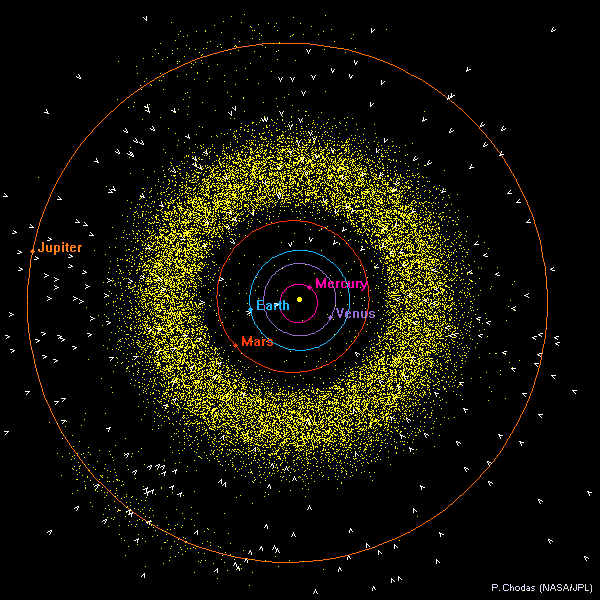
\includegraphics[width=0.5\linewidth, height=\textheight, keepaspectratio=true]{asteroid_distribution_orbit_plot_inverted.png}
        \label{fig:inner_asteroids}
        }
    }
    \subfloat[]{
        \fbox{
        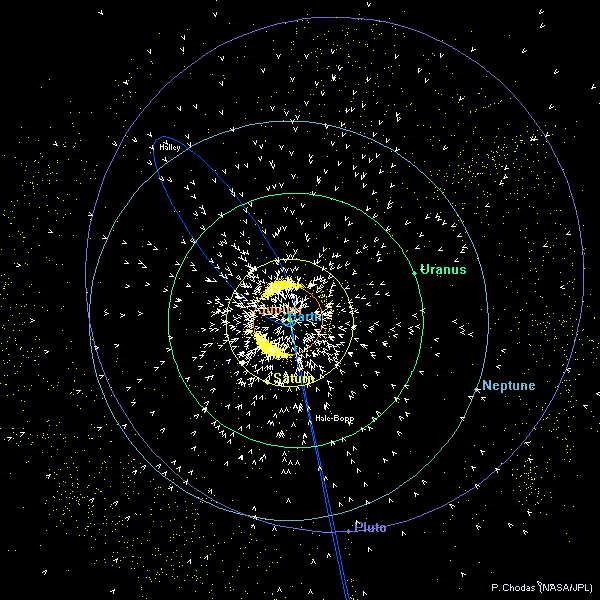
\includegraphics[width=0.5\linewidth, height=\textheight, keepaspectratio=true]{asteroid_distribution_outer_orbit_plot_inverted.png}
        \label{fig:outer_asteroids}
        }
    }
\caption{Distribution of asteroids in \protect\subref{fig:inner_asteroids} inner Solar System and \protect\subref{fig:outer_asteroids} outer Solar System. Asteroid locations are shown by blue-colored dots whereas the black-colored wedges pointing towards the Sun represent the comets. The diagrams are based on the small-bodies cataloged up until November 2016 \parencite{jpl_asteroid_web}. These images are color-inverted versions of the original.}
\label{fig:asteroid_distribution}
\end{figure}
\FloatBarrier
%%%
Two more asteroid rendezvous missions launched quite recently are of particular interest to this thesis. Following the success of Hayabusa, \gls{JAXA} launched another sample return mission called Hayabusa-2 to asteroid 1999 JU3, scheduled to be in orbit around it by mid-2018. It will perform a 1.5 year long close-proximity operation at the asteroid that includes surface sample acquisition, which will eventually be returned to Earth in a capsule, and a \SI{2}{\metre} wide cratering event to observe the sub-surface \parencite{TsudaHayabusa2SystemDesign}. The \gls{OSIRIS-REx} mission by \gls{NASA}, directed towards asteroid Bennu and scheduled to enter into an orbit around it in late 2018, will also retrieve a surface sample and return it back to Earth. It will employ a \gls{TAG} maneuver to acquire a sample within a 1.5 month long scheduled sampling period \parencite{berry2013osiris}. Both missions are aiming to find out if organic material, volatiles and water itself were brought to Earth by such asteroids. These missions employ techniques for sample acquisition that could potentially disturb the state of regolith on the surface of the asteroid and loft it into an orbit. Even without any spacecraft interaction, material can be lofted from the surface of an asteroid due to meteoroid impacts. In either case, it is imperative to understand the complex dynamical environment around asteroids, not only for spacecraft operations and safety, but also to learn about the orbital motion of lofted regolith and its eventual fate. \gls{NASA} has identified the acquisition of such information as a \gls{SKG} for \glspl{NEO}, specifically article III-A-1: Expected particulate environment due to impact ejecta in \cite{nasa_skg}.
%
\newline\newline
%
Regolith is defined as fine and loosely held rock which covers bedrock and constitutes the surface of a celestial body. The study of lofted regolith around an asteroid is by no means a new research topic. In the studies done previously \parencite{richter1995stability,lee1996dust,scheeres1996orbits,scheeres2000ejecta,korycansky2004_impactEjecta,yarnoz2014passive}, we have witnessed certain minor drawbacks. For instance, not always accounting for gravity and Solar perturbations together; using an approximated analytical method to understand the dynamical environment that falls short on obtaining the entire spectra of initial conditions that could lead to different final outcomes (re-impact, escape or temporary capture) for lofted regolith; not considering different sizes and densities for the lofted regolith; and finally, not considering the local direction with respect to a rotating asteroid in which the regolith is ejected. This thesis, thus, aims to address these shortfalls in a single study, and by using numerical simulation techniques, to add more fidelity in understanding what happens to regolith when it is lofted from the surface of an asteroid.
%
\newline\newline
%
The study of orbiting regolith is important for understanding the displacement of material on surface of the asteroid in case of natural or spacecraft-induced impact cratering events. From a mission design point-of-view, the ejecta from an impact cratering event could pose a serious threat to spacecraft and/or its instruments. By knowing the orbital behavior of regolith in advance, mission designers can make informed decisions on the trajectory design of spacecraft to avoid or reduce failure scenarios. Another important benefit that comes from a study like this is in the field of asteroid mining, whereby the regolith's orbital motion and final fate can be exploited to sort different materials in real time. The results from this thesis will thus aid mission designers in planning future asteroid missions and in answering the following research question:
\vspace{5mm}
%%%
\begin{center}
    \fbox{\parbox{0.8\textwidth}{
    \centering
    \textbf{\textit{Can we explain the orbital behavior and eventual fate of lofted regolith around an asteroid in presence of gravity and Solar perturbations?}}}
    }
\end{center}
%%%
\vspace{5mm}
The structure of this report is mentioned as follows: \Cref{chap:heritage} briefly discusses the past and the future missions to asteroids in the context of this thesis, and a few research publications that are relevant for our work. This paves the way to define the research questions and goals in \Cref{chap:research_questions}. \Cref{chap:dynamics_modeling} discusses the models for simulating an asteroid's gravity and the Solar perturbations, equations of motion for the regolith and its launch conditions, and finally a non-conservative algorithm to determine a regolith's guaranteed escape speed. The verification and validation of the simulation models can be found in \Cref{chap:v_and_v}. \Cref{chap:nonconservative} discusses the performance of the conservative guaranteed escape speed algorithm for a spherical and an ellipsoidal asteroid and the performance of the non-conservative algorithm for the ellipsoidal asteroid. \Cref{chap:dynamics_without_solar_perturbations} discusses the general characteristics of lofted regolith and its final fate for an ellipsoidal asteroid in the absence of Solar perturbations. \Cref{chap:dynamics_with_solar_perturbations} does the same analysis but in the presence of Solar perturbations and for regoliths of different size and density. \Cref{chap:conclusions} summarizes all the results by presenting answers to all the sub-research questions from \Cref{chap:research_questions}. Finally, \Cref{chap:recommendations} provides some recommendations for future work on our research topic.

% Asteroids are not only found as single, isolated bodies in the Solar System, but also as multi-body local systems consisting of two or three asteroids. Over 190 multiple asteroid systems have so far been detected in the Solar System. They are significantly diverse in terms of the size ratios of the individual asteroids, their orbit motion and separation around each other, implicating that the individual asteroids evolved differently over time \parencite{multipleAsteroids}. If two or three asteroids are bound to each other gravitationally, then they are termed as \textit{binary asteroids} and \textit{triple asteroids} respectively. An example of a binary asteroid system is shown in \Cref{fig:ida_dactyl_image}. However, if individual asteroids share similar heliocentric orbits but are not gravitationally bound to each other, then they are termed as \textit{asteroid pairs}. Within a pair, if the larger asteroid is itself a binary or a triple asteroid system, then the pair is termed as \textit{paired binary} or \textit{paired triple} respectively \parencite{multipleAsteroidsTerminology}. Asteroids can further be classified into categories based on their dimensions and thermal properties, and is discussed in \cite{multipleAsteroids}.

\part{Motivation}
\chapter{Heritage}
\label{chap:heritage}
\graphicspath{{Mission_Heritage/Images/}}

In the past, there have been multiple spacecraft missions to the small bodies in our Solar System which have collectively increased our understanding about them. While a large majority of these have been asteroid fly-by scenarios, a few have also been rendezvous missions \parencite{esa_mission2asteroids_web}. This chapter will provide an overview on few of these missions followed by a brief literature review which shall be of interest to the thesis at hand. This will help us in justifying the research objectives mentioned in \Cref{chap:research_questions}. \Cref{sec:past_missions} will discuss the asteroid rendezvous missions which have already taken place, \Cref{sec:future_missions} will discuss future rendezvous missions, and finally, \Cref{sec:literature_review} will discuss the state-of-the-art.

\section{Past Missions}
\label{sec:past_missions}
In all the history of space exploration there have been only three spacecraft missions that have rendezvoused with asteroids. In chronological order these are: \gls{NASA}'s \gls{NEAR}-Shoemaker mission to asteroid Eros, \gls{JAXA}'s Hayabusa mission to asteroid Itokawa, and \gls{NASA}'s Dawn mission to asteroids Vesta and Ceres \parencite{scheeresBook}. Out of these, only \gls{NEAR} and Hayabusa had direct contact with the small bodies and acquired high-resolution imagery of surface regolith.

\subsection{NEAR-Shoemaker}
\label{subsec:near_heritage}
The \gls{NEAR}-Shoemaker (henceforth \gls{NEAR}) mission was launched in 1996 and rendezvoused with Eros in 2000. Its operational phase around the asteroid continued for about a year during which it obtained several high-resolution images of the surface and collected comprehensive measurements to estimate its internal mass distribution, shape model, gravity and spin state amongst other observations \parencite{scheeresBook}. The bulk density of Eros was estimated to be $2.67 \pm 0.03 [g/cm^3]$ and its mass to be $(6.6904 \pm 0.003) \times 10^{15} [kg]$. The rotation state was estimated to be $1639.38922 \pm 0.00015$ [deg/day] which gives a rotational period of about $5.27$ [hrs] \parencite{erosShapeDetermination}. On 25 October 2000, \gls{NEAR} executed a \gls{LAF} over Eros in which it acquired several high-resolution images that helped in understanding the surface morphology. The images confirmed the existence of a substantial amount of regolith on the surface with a typical thickness value of tens of metres over the bedrock, except of course on steep slopes. The regolith was found to be highly complex, in that it varied from fine material to metre-sized ejecta blocks \parencite{Veverka2001}. \cite{Robinson2001} estimates the size of the finer regolith to be around 1.0 [cm] or smaller from images that had a resolution of 1.2 [cm] per pixel. \Cref{fig:eros_regolith} depicts the regolith morphology in one of the high-resolution imaging sequences from the \gls{LAF} \parencite{veverka2001landing}.
%%%
\begin{figure}[htb]
\centering
\captionsetup{justification=centering}
\includegraphics[width=\linewidth, height=0.5\textheight, keepaspectratio=true]{eros_regolith.pdf}
\caption{Mosaic of high-resolution images depicting the nature of regolith on the surface of Eros \parencite{veverka2001landing}.}
\label{fig:eros_regolith}
\end{figure}
\FloatBarrier
%%%

\subsection{Hayabusa}
\label{subsec:hayabusa_heritage}
The Hayabusa spacecraft was launched by \gls{JAXA} in 2003 and it arrived at asteroid Itokawa in 2005. After arrival, it performed close-proximity operations around the asteroid for approximately 3 months during which several measurements were taken to estimate the shape, mass, topography and elemental composition of the asteroid. During this period, the spacecraft also collected samples from the surface of the asteroid that were eventually returned back to Earth in 2010. The measurements at Itokawa estimated its mass to be $3.51 \times 10^{10}$ [kg] and its bulk density to be $1.9 \pm 0.13$ [g/$cm^3$] \parencite{fujiwara2006ItokawaHayabusa}.
%
\newline\newline
%
Two distinct types of terrains can be recognized on Itokawa, one which is rough and rich in boulders and the other which is smooth and mostly flat. This distinction can easily be seen in \Cref{fig:itokawa_regolith}. The smooth regolith regions, that account for approximately 20\% of Itokawa's surface, composed of fragmented debris with grain sizes ranging from sub-centimetre to centimetre scales. One of the smooth regolith regions, called Muses Sea and from where the sample was also acquired, even consisted of a few metre-sized boulders that were hypothesized to have landed in the region as secondary ejecta \parencite{miyamotoItokawaRegolith}. The rougher terrain on Itokawa, which has a very sharp boundary with the smoother regolith filled regions (as evident in \Cref{fig:itokawa_regolith}), consists of boulders that range upto tens of metres in size \parencite{fujiwara2006ItokawaHayabusa}.
%%%
\begin{figure}[htb]
\centering
\captionsetup{justification=centering}
\includegraphics[width=\linewidth, height=0.5\textheight, keepaspectratio=true]{itokawa_regolith.pdf}
\caption{Image of Itokawa taken from a 7 [km] altitude depicting the nature of regolith on its surface. Muses Sea and Sagamihara are the two distinct smooth regolith regions on the asteroid \parencite{fujiwara2006ItokawaHayabusa}.}
\label{fig:itokawa_regolith}
\end{figure}
\FloatBarrier
%%%
Hayabusa employed an \textit{impact sampling mechanism} that would work across various types of terrains, from hard bedrock to fine regolith. The spacecraft consisted of a long cylindrical sampling horn with a conical tip. When the tip of the horn touched the surface of the asteroid, the deformation in the horn's fabric was detected by a laser range finder and within 0.3 [s] of this event, a 5.0 [g] projectile was fired towards the surface with a velocity of 300 [m/s] and the resultant ejecta was collected by the sampler \parencite{yano2004sampling}. \cite{yanoHayabusaTouchdown} presents data from the sampling experiments that were performed on ground in $1g$ and micro-gravity environments. The experiments revealed that, for the projectile hitting at normal impact angles in micro-gravity, the impact ejecta mass of particles greater than 1.0 [cm] ranged from 2 - 11 [g] whereas for particles less than 1.0 [mm] the ejecta mass ranged from 100 - 10000 [g]. The impact target consisted of various analog materials from glass beads to lunar regolith simulant and an experiment like is a nice indicator of how artificial impact events can displace significant amount of fragmented debris on an asteroid.

\section{Future Missions}
\label{sec:future_missions}
We will now discuss two missions, Hayabusa-2 by \gls{JAXA} and \gls{OSIRIS-REx} by \gls{NASA}. Both are currently en route to their respective target asteroids and after orbit insertion, they shall perform operations to collect surface samples.

\subsection{Hayabusa-2}
\label{subsec:hayabusa2_heritage}
Hayabusa-2 is the second asteroid sample return mission by \gls{JAXA}, which to a significant extent, shares the successful technical legacy of Hayabusa. The target asteroid of the former is \textit{1999 JU3} which is suspected to contain organic matter and hydrated minerals. A successful sample return from this asteroid may thus help us in understanding the origin of life and/or water on Earth. The spacecraft will enter into an orbit around its target by mid-2018, after which it will perform close-proximity operations for 1.5 years. The mission will entail 3 touchdowns for sample acquisition and a cratering event to observe the subsurface of the asteroid. The sampling mechanism is based on that of Hayabusa and each sampling attempt has the potential to acquire samples in the order of 100 [mg]. The samples are sealed-off and transported back to Earth in a re-entry capsule. The cratering operation is performed by a \gls{SCI}. The \gls{SCI} is deployed by the spacecraft at an altitude of 500 [m] and after a preset time, a detonation accelerates it to about 2 [km/s] prior to impact. It is estimated that this will result in a crater of about 2 [m] wide. Prior to the detonation of \gls{SCI}, the spacecraft will move to a safe location on the opposite side of the asteroid from the impact point to avoid damage from impact ejecta and/or debris from the detonation. Apart from these, the spacecraft will perform other in-situ operations to characterize the asteroid and will also deploy a lander and three miniature rovers for technology demonstration \parencite{TsudaHayabusa2SystemDesign}.

\subsection{OSIRIS-REx}
\label{subsec:osiris_heritage}
\gls{OSIRIS-REx} is part of \gls{NASA}'s New Frontiers program and will travel to \gls{NEA} 1999 $RQ_{36}$, also known as Bennu. The mission, amongst other scientific objectives, will return a regolith sample back to Earth that may provide insight into the initial states of planetary formation as well as answer questions on the origins of life. Since Bennu is a \gls{NEA}, the sample collection and subsequent analysis will provide us information on asteroids that could potentially impact Earth. The spacecraft was launched in 2016 and is expected to reach its target by the end of 2018 \parencite{berry2013osiris}. The asteroid has a semi-major axis of 1.126 [AU] which makes it an easily accessible asteroid as far as distance is concerned. But more than that, Bennu falls under the category of asteroids that are rich in volatiles and could potentially be related to objects that brought the seeds of life to Earth. Initial observations of Bennu through ground based telescopes, the Spitzer Telescope, the Arecibo Observatory and other assets revealed an abundance of regolith on the surface with grain sizes ranging from 4 - 8 [mm]. \gls{OSIRIS-REx} will acquire the regolith sample using a \gls{TAG} mechanism which uses pressurized Nitrogen gas to force the loosely held regolith into a collection chamber. The sampling will occur in 2020 and it will be retrieved on Earth in 2023 \parencite{osirisMissionOverview}.

\section{State of the art / Literature Review}
\label{sec:literature_review}

\chapter{Research Questions \& Goals}
\label{chap:research_questions}
\graphicspath{{Research_Questions/Images/}}

The study of the dynamics of a particle, on or around an asteroid, can be broadly divided into three main regimes. The first regime involves the study of surface ejecta generation, from natural events such as interplanetary particle impacts, cratering by other asteroids \& electrostatic dust levitation, or from space exploration events where the natural state of the regolith is disturbed by spacecraft sampling activities. The second regime involves the study of the subsequent orbital behavior of impact ejecta or lofted regolith under varying parameters such as launch conditions, asteroid rotational state \& shape, regolith particle size and density, Solar phase etc. And finally, the third regime involves the study of particle dynamics when it re-impacts with the surface of the asteroid. This thesis will concern itself with the second regime of research, i.e., the natural orbital evolution of regolith lofted from an asteroid’s surface.
%
\newline\newline
%
As mentioned earlier in \Cref{chap:intro}, understanding particulate environment around small-bodies has been identified by \gls{NASA} as a strategic knowledge gap. Understanding and developing tools or knowledge to estimate the orbital behavior and final fate of lofted regolith with greater accuracy is important for future space exploration missions (see \Cref{sec:future_missions}) that will involve direct interactions with asteroids, to avoid any damage to the spacecraft or surface robotic crew from orbiting particles. High-fidelity simulations of particulate motion can also help scientists in understanding the surface morphology of asteroids by helping them recreate cratering events. In \Cref{sec:literature_review}, we highlighted the shortfalls in the research done on the topic so far and we identified a gap that needs to be filled, and hence, the following top level research question is set:
\vspace{5mm}
%%%
\begin{center}
    \fbox{\parbox{0.8\textwidth}{
    \centering
    \textbf{\textit{Can we explain the orbital behavior and eventual fate of lofted regolith around an asteroid in presence of gravity and Solar perturbations?}}}
    }
\end{center}
%%%
\vspace{5mm}
This top-level research question is divided into the following sub-questions that help in structuring the thesis:
%%%
\begin{enumerate}
\item Does the regolith, launched from different locations such as leading, trailing, longest and shortest edge of an asteroid, show characteristic differences with regard to its final fate?
\item Can clear demarcation be established between the re-impact, capture, and escape scenarios, for the lofted regolith, based solely on the initial conditions?
\item What causes the regolith to enter into a temporary capture orbit around the asteroid?
\item For the same launch conditions, how does the orbital behavior and final fate of the regolith differ for different particle sizes and densities?
\item For the same particle size and density, how does the orbital behavior and final fate change with different launch locations?
\item Can we establish a non-conservative analytical expression to determine guarantee escape speed in presence of perturbations?
\item Can we exploit the orbital behavior of lofted regolith for sorting material of different sizes and densities as an application for asteroid mining?
\end{enumerate}
%%%
\vspace{5mm}
In order to answer these questions, the following main research goal is set:
%%%
\begin{center}
    \fbox{\parbox{0.8\textwidth}{
    \centering
    \textbf{\textit{Investigate the orbital motion of regolith launched from the surface of an asteroid using numerical simulations.}}}
    }
\end{center}
%%%
The sub-research goals are mentioned as follows:
%%%
\begin{enumerate}
\item Develop a modular and robust software tool that can propagate the trajectory of spherical particles around an asteroid for given initial conditions.
\item Develop software tools to plot and analyze numerical simulation results
\item Validate the software tools.
\item Perform simulations for particles launched from the asteroid's surface with different initial conditions, launch locations, and for different particle sizes \& densities.
\item Perform qualitative and quantitative analysis on numerical simulation results.
\item Document results and inferences for thesis report and peer reviewed journal paper.
\end{enumerate}
%%%
The vast majority of the time will be spent on designing the simulator and data processing \& visualization tools (see \Cref{chap:naos}), followed by their verification and validation (see \Cref{chap:v_and_v}). A relatively smaller time would then remain to perform the research and investigate the results, however the time remaining for this would be sufficient to answer all our research questions.

\part{Dynamics Modeling \& Simulator}
\chapter{Orbital dynamics around Asteroids}
\label{chap:dynamics_modeling}
\graphicspath{{Modeling/Images/}}

This chapter will focus on accurate modeling of the asteroid environment and the equations of motion of a particle around it in presence of gravitational and Solar perturbations.

\section{Modeling Assumptions}
\label{sec:assumptions}
Every research involves some degree of approximation of the natural world, on Earth or otherwise, to understand or explain any phenomenon. Through this thesis work, we hope to understand the orbital behavior of regolith around an asteroid and we have to do it with a relatively simplified model because recreating an exact replica of an asteroid's dynamical environment is out of the scope of this thesis. Although we are making simplifications, but it does not mean that the . Thus we make certain simplifying assumptions while modeling the asteroid-regolith system and these are mentioned as follows:
%%%
\begin{enumerate}
\item The asteroid body is modeled as a smooth triaxial ellipsoid to account for its non-uniform gravity. The reasons for choosing this model over others will be explained later in \Cref{sec:gravity}.

\item Craters, surface depressions, mountains or any other terrain deformity on the asteroid is not considered in the simulation. The body is considered to have a uniform density. This is to simplify calculations of the gravitational acceleration.

\item The asteroid is rotating uniformly about its shortest axis. This is considered for simplicity and also because most Solar System bodies would dissipate energy to eventually enter a rotational state that is uniform and about its axis of maximum moment of inertia \parencite{scheeresBook}.

\item The regolith grains are assumed to be of spherical shape to simplify the \gls{SRP} calculation as the cross-sectional area of a sphere would remain the same irrespective of its attitude.

\item Multiple regolith particles are launched from a given location on the asteroid in the form of a cone to replicate ejecta from a cratering event. But all particles are assumed to be coming off from the same point, unlike that in the case of an actual cratering event. This is because the pretext of the thesis was that the regolith is lofted due to an activity from a spacecraft and such would result in relatively smaller craters (from artificial cratering events) or surface depressions. Thus assuming that all particles in this \textit{"ejecta cone"} emerge from the same point on the asteroid is reasonable and simplifies the simulation.

\item The slant angle of the \textit{"ejecta cone"} (henceforth the declination angle) from the local surface normal is kept constant at 45.0 [deg] (which is a middle value in the entire declination range from 0.0 - 90.0 [deg]). We want to consider a general case and not introduce another degree-of-freedom in terms of varying declination angles.

\item The loss of material and mass from the asteroid, when the regolith is lofted from the surface, is not modeled in the simulation since it is assumed that a very small amount of material will be displaced by a spacecraft activity. This assumption is based on the sample collected by the Hayabusa mission (see \Cref{sec:past_missions} and the references therein).

\item Interaction between individual regolith grain is not accounted for because we are simulating multiple particles being lofted at the same time and granular interaction on such a scale would be extremely complex and beyond the scope of this thesis.

\item Secondary motion of regolith, after re-impacting the surface is not modeled and it is assumed that the particles just come to a standstill.

\item The shadow region of the asteroid is not modeled which means that the solar perturbations are always acting on the regolith grain and this simplification was made since asteroids are extremely small compared to planets, and thus the orbiting particles wouldn't spend long periods of time in the shadow.

\item Perturbations are considered only from the Sun. \gls{SRP} is important because regolith grains will have higher Area-To-Mass ratios, relative to a spacecraft, and so the radiation pressure would be significantly large for them. We model the third body attraction from the Sun (\gls{STBE}) as well but not from any of the giant planets such as Jupiter or Saturn, because the magnitude of perturbation from the \gls{STBE} itself is atleast 5 orders of magnitude smaller than the gravitational acceleration when the regolith is in close proximity to the asteroid (see \Cref{chap:results}).

\item The apparent motion of the Sun around the asteroid is considered circular and in the equatorial plane of the asteroid. "Refer to the two papers here talking about inclination and sma of MBO".
\end{enumerate}
%%%

\section{Reference Frames}
\label{sec:reference_frames}
Before describing the motion of regolith around the asteroid, its important to define the frames of reference with respect to which this motion is defined and the transformation of state vectors between these frames. We use two asteroid centric reference frames, both of which are depicted in \Cref{fig:reference_frame}. Since we will be using a triaxial ellipsoid to model an asteroid (for details, see \Cref{sec:gravity}), the body-fixed rotating frame with respect to this model is shown in \Cref{fig:ellipsoid_rotating_frame}.
%%%
\begin{figure}[htb]
\centering
\captionsetup{justification=centering}
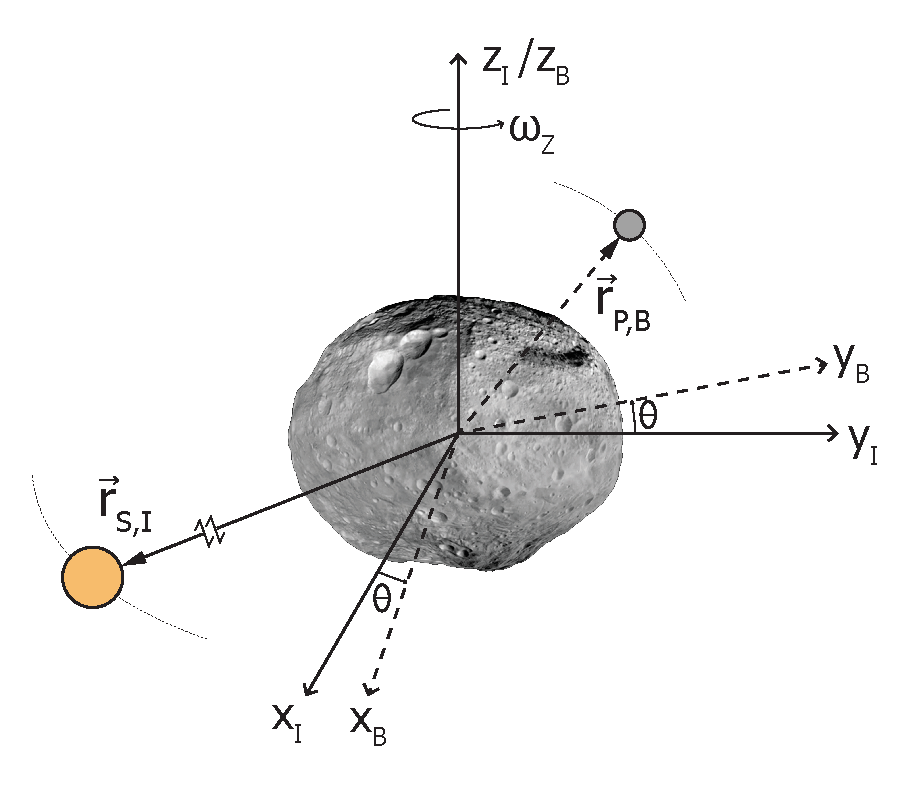
\includegraphics[width=\textwidth, height=0.35\textheight, keepaspectratio=true]{reference_frames.pdf}
\caption{The diagram depicts two asteroid centric reference frames, one being Inertial (depicted by solid line and the subscript \emph{I}) and the other being a body-fixed Rotating frame (denoted by dashed line and the subscript \emph{B}). The position vector to a regolith particle is shown as $\protect\vv{\bm{r}}_{P,B}$, whereas the position vector to the Sun from the asteroid is shown as $\protect\vv{\bm{r}}_{S,I}$.}
\label{fig:reference_frame}
\end{figure}
\FloatBarrier
%%%
%%%
\begin{figure}[htb]
\centering
\captionsetup{justification=centering}
\includegraphics[width=\textwidth, height=0.35\textheight, keepaspectratio=true]{body_fixed_ellipsoid_frame.pdf}
\caption{Representation of the body-fixed rotating frame for a triaxial ellipsoid model of an asteroid. $\bm{x_{B}}$ is aligned with the longest axis, $\bm{z_{B}}$ is aligned with the shortest axis and $\bm{y_{B}}$ is aligned with the remaining last axis of the ellipsoid.}
\label{fig:ellipsoid_rotating_frame}
\end{figure}
\FloatBarrier
%%%
The two frames are defined as follows:
%%%
\begin{enumerate}
\item \gls{AIF} - This is a non-rotating frame fixed inertially in space with its origin at the centre of mass of the asteroid . \Cref{fig:solar_phase_and_inertial_frame} shows the orientation of the frame (in \emph{x-y} plane) such that the \emph{x-axis} is pointing to the Sun when the Longitude of the Sun (or effectively the True Anomaly of the apparent circular motion of the Sun around the asteroid) ($\vartheta$) is zero. The \emph{y-axis}, thus, points to the sun when $\vartheta = 90^o$ and finally the \emph{z-axis} is obtained by following the right-hand rule, coming out of the sheet in 3D.
%
\item \gls{ARF} - This frame is fixed to the rotating asteroid with its origin at the centre of mass of the asteroid. \Cref{fig:ellipsoid_rotating_frame} shows the orientation of this frame, assuming a triaxial ellipsoid model for our asteroid (for details see \Cref{sec:gravity}). The \emph{x-axis} is pointing along the longest axis of the triaxial ellipsoid, and the \emph{y-axis} is pointing along the shortest axis of the ellipsoid. The \emph{y-axis} points in a direction so as to complete the right-hand rule
\end{enumerate}
%%%
%%%
\begin{figure}[htb]
\centering
\captionsetup{justification=centering}
\includegraphics[width=\textwidth, height=0.35\textheight, keepaspectratio=true]{solar_phase_and_inertial_frame_3.pdf}
\caption{Asteroid-centric inertial frame \emph{x-y} plane. The position vector to the Sun is shown as $\protect\vv{\bm{r}}_{S,I}$. The apparent motion of the Sun around the asteroid, assumed a circular orbit, is also depicted with $\vartheta$ as the Longitude of Sun (or effectively the True Anomaly). The four phases are for a broader identification of the Sun's location with respect to the asteroid.}
\label{fig:solar_phase_and_inertial_frame}
\end{figure}
\FloatBarrier
%%%

\section{Gravity Modeling}
\label{sec:gravity}
...elliptic integral method and how the accelerations are calculated and the third order equation solving for lambda...

\section{Solar Perturbations}
\label{sec:solar_perturbations}

\section{Perturbed Two-Body Problem}
\label{sec:2BP}

\section{Particle Initial Conditions}
\label{sec:init_conditions}
...launch velocity, location and direction calculation...

\section{Non-conservative Escape Speed}
\label{sec:escape_speed_derivation}

\section{Conclusion}
\label{sec:dynamics_conclusion}

\chapter{NAOS: Near-Asteroid Orbit Simulator}
\label{chap:naos}
\graphicspath{{NAOS/Images/}}

\chapter{Verification \& Validation}
\label{chap:v_and_v}
\graphicspath{{V&V/}}

In this chapter, we will present the results on verification and validation of the simulator discussed in \Cref{chap:naos}. We verify the gravity model, the launch conditions for the regolith, the numerical integrator along with the equations of motion for the regolith, and finally the Solar perturbation models. We validate our simulator to ensure that our inferences for any scientific result out of it remains true and valid as well.

\section{Constant Density Ellipsoid Gravity Model}
\label{sec:gravity_vv}
The \gls{CDE} gravity model was tested for a singular target point by comparing the gravitational potential and acceleration values at that point as computed by \gls{NAOS}, with external data obtained from another researcher at CSML \footnote{Centre for Spaceflight Mechanics Laboratory; The thesis work was partly done at CSML, which is a research lab headed by Dr. Daniel Scheeres and is part of the University of Colorado, Boulder, USA.}. The parameters used for the test are given in \Cref{tab:gravity_vv_params}.
%%%
\begin{table}[htb]
\centering
\captionsetup{justification=centering}
\caption{Parametric values used for testing the \gls{CDE} gravitational potential model.}
\label{tab:gravity_vv_params}
\begin{tabular}{|l|l|l|}
\hline
\multicolumn{1}{|c|}{\textbf{Parameter}} & \multicolumn{1}{c|}{\textbf{Value}} & \multicolumn{1}{c|}{\textbf{Units}}      \\ \hline
Gravitational Parameter                  & 446382.0                            & \si{\metre \cubed \per \second \squared} \\ \hline
Alpha (longest axis of \gls{CDE})      & 20000                               & \si{\metre}                            \\ \hline
Beta (Intermediate axis of \gls{CDE})  & 7000                                & \si{\metre}                            \\ \hline
Gamma (Shortest axis of \gls{CDE})     & 7000                                & \si{\metre}                            \\ \hline
Target point x-coordinate                & 10000                               & \si{\metre}                            \\ \hline
Target point y-coordinate                & 13000                               & \si{\metre}                            \\ \hline
Target point z-coordinate                & 8000                                & \si{\metre}                            \\ \hline
\end{tabular}
\end{table}
\FloatBarrier
%%%
The test values for the gravitational potential and the acceleration values at the specified target point are given in \Cref{tab:gravity_vv_test_values}.
%%%
% Please add the following required packages to your document preamble:
% \usepackage{multirow}
\begin{table}[htb]
\centering
\captionsetup{justification=centering}
\caption{Test values for verification of the \gls{CDE} gravity model.}
\label{tab:gravity_vv_test_values}
\begin{tabular}{|l|l|l|l|}
\hline
\multicolumn{1}{|c|}{\textbf{Parameter}}    & \multicolumn{2}{c|}{\textbf{Value}}     & \multicolumn{1}{c|}{\textbf{Units}}          \\ \hline
Gravitational Potential                     & \multicolumn{2}{l|}{23.710052554396402} & \si{\metre \squared \per \second \squared} \\ \hline
\multirow{3}{*}{Gravitational Acceleration} & x       & -0.00044762916738340803       & \si{\metre \per \second \squared}          \\ \cline{2-4}
                                            & y       & -0.0009623388813999501        & \si{\metre\per \second \squared}           \\ \cline{2-4}
                                            & z       & -0.000592208542399969         & \si{\metre\per \second \squared}           \\ \hline
\end{tabular}
\end{table}
\FloatBarrier
%%%
The values obtained from the simulator \gls{NAOS} were compared with the ones in \Cref{tab:gravity_vv_test_values} upto the 12th decimal point and they matched, validating the gravity model implemented in \gls{NAOS}.

\section{Regolith Launch Conditions}
\label{sec:regolith_launch_conditions_vv}
In this section, we'll presents results on verifying whether the initial state vector for the regolith or the launch condition match to what is desired by the user. Here, an internal validation is done to ensure that the launch conditions registered in the output database match the raw value input to \gls{NAOS}. We present graphical and numerical results in this regard.

\subsection{Launch Location}
\label{subsec:launch_location_vv}
The position vector to the launch location, from the centre of the \gls{ARF}, is formed by giving only the launch location latitude and longitude as input. Thus, we have to verify whether the position vector conforms to a given angular input. We take the initial state vector, from the output databases of the dynamics simulator, of regolith launched from a few launch locations on the asteroid and convert the Cartesian coordinates back to latitude and longitude to see if the position vector was formed correctly. For the same Cartesian coordinates, we use the triaxial ellipsoid equation, and see if they solve the equation, to verify that the launch point lies on the surface of the asteroid.
%
\newline\newline
%
We took 5 test locations from where regolith was launched and separately calculated the corresponding longitude and latitude for the launch location to check if the position vector was correctly formed. The position coordinates and the back-calculated latitude and longitude angles are shown in \Cref{tab:position_vector_to_lat_long_vv}.
%%%
\begin{table}[htb]
\centering
\captionsetup{justification=centering}
\caption{Position vector to different launch locations and the corresponding Latitude and Longitude angles.}
\label{tab:position_vector_to_lat_long_vv}
\begin{tabular}{|c|c|c|c|c|}
\hline
\textbf{X {[}m{]}} & \textbf{Y {[}m{]}} & \textbf{Z {[}m{]}} & \textbf{Longitude {[}deg{]}} & \textbf{Latitude {[}deg{]}} \\ \hline
20000.0 & 0.0 & 0.0 & 0.0 & 0.0 \\ \hline
0.0 & 7000.0 & 0.0 & 90.0 & 0.0 \\ \hline
0.0 & 0.0 & 7000.0 & 0.0 & 90.0 \\ \hline
3316.14545023 & 1914.57746836 & 6632.29090046 & 30.0 & 60.0 \\ \hline
-3961.38284482 & -3961.38284482 & 5602.2413449 & -135.0 (225.0) & 45.0 \\ \hline
\end{tabular}
\end{table}
\FloatBarrier
%%%
The longitude and latitude values given in \Cref{tab:position_vector_to_lat_long_vv} were calculated from the Cartesian coordinates and match those given as inputs to the dynamics simulator. The position vectors from \Cref{tab:position_vector_to_lat_long_vv} with the \gls{CDE} model are also depicted in \Cref{fig:position_vector_diagram}.
%%%
\begin{figure}[htb]
\centering
\captionsetup{justification=centering}
\subfloat[]{
    \includegraphics[width=\textwidth, height=0.4\textheight, keepaspectratio=true]{Images/launch_location_position_vectors.pdf}
    \label{fig:launch_location_vv_1}
    }

\subfloat[]{
    \includegraphics[width=\textwidth, height=0.4\textheight, keepaspectratio=true]{Images/launch_location_position_vectors_2.pdf}
    \label{fig:launch_location_vv_2}
    }
\caption{Position vectors from \protect\Cref{tab:position_vector_to_lat_long_vv} shown with the \protect\gls{CDE} asteroid model.}
\label{fig:position_vector_diagram}
\end{figure}
\FloatBarrier
%%%
We also checked whether the launch location in fact did lie exactly on the surface of the \gls{CDE} asteroid and not inside or above the surface. This is really important because a wrong initial condition could produce erroneous results. Once we substitute the Cartesian coordinates into the triaxial ellipsoid equation (see \Cref{eqn:launch_loc_ellipsoid_eqn_cartesian}) and if the output equals zero (when we take the term 1.0 on the right hand side in \Cref{eqn:launch_loc_ellipsoid_eqn_cartesian}), then the launch point lies on the asteroid. We did an external validation for this but an internal validation always takes place within the dynamics simulator at all times whenever a new simulation is run.
%%%
\begin{table}[htb]
\centering
\captionsetup{justification=centering}
\caption{Output of the triaxial ellipsoid equation for a few test launch location position vectors. An output of 0.0 means that the position vector is a perfect root of the equation and hence the launch location indeed lies on the surface of the asteroid.}
\label{tab:launch_location_surface_vv}
\begin{tabular}{|c|c|c|c|}
\hline
\textbf{X {[}m{]}} & \textbf{Y {[}m{]}} & \textbf{Z {[}m{]}} & \textbf{Output of triaxial ellipsoid equation} \\ \hline
20000.0 & 0.0 & 0.0 & 0.0 \\ \hline
0.0 & 7000.0 & 0.0 & 0.0 \\ \hline
0.0 & 0.0 & 7000.0 & 0.0 \\ \hline
3316.14545023 & 1914.57746836 & 6632.29090046 & 2.22044604925e-16 \\ \hline
-3961.38284482 & -3961.38284482 & 5602.2413449 & 0.0 \\ \hline
\end{tabular}
\end{table}
\FloatBarrier
%%%

\subsection{Launch Velocity}
\label{subsec:launch_velocity_vv}
The launch velocity vector is formed by providing two angles and a magnitude. As explained in \Cref{subsec:launch_velocity}, the two angles are the declination angle from the normal vector at the launch location and the azimuth angle from the local North direction. The local North direction and the normal vector, in essence, act as the basis vectors for a local surface frame of reference which in turn help in the mathematical formulation of the velocity vector of Cartesian components. Since we are dealing with an ellipsoid and not a sphere, defining local North is not a straight-forward process as explained earlier in \Cref{subsec:launch_velocity}.
%
\newline\newline
%
Thus, we first begin with verifying our methodology of forming the local surface frame, and ensure that the local Normal vector and the local North pointing vector are correctly formed and their lies no discrepancy. Then we verify whether the velocity vector, in terms of its Cartesian components, indeed makes the same angle with the surface frame as specified at the input of the simulation. The process for the second verification item is different from how the velocity vector was formed in the first place and hence the verification itself won't be a tampered or faulty process.
%
\newline\newline
%
Let's first begin with a test launch location at the longest edge of the \gls{CDE}. A graphical depiction of the frame is shown in \Cref{fig:surface_frame}. This is the simplest location to perform any simulation or test because the surface normal vector here will be along the same direction as the position vector to the launch point from the centre of the ellipsoid. This also makes the test in itself a trivial task. Note that the surface normal is also the z-axis for the surface frame at the launch point. So for the current test location, if the cross product of the normal and the position vector is a zero vector, then the normal vector is verified. \Cref{tab:longest_edge_surface_frame_vv} shows the result for this. Following this, if the angle between the normal vector and the x-axis basis vector for the surface frame is \SI{90}{\degree}, then the latter is pointing to the local North direction. This is because for the current test location, any vector perpendicular to the surface normal (or effectively to the launch location position vector) will be along the \SI{0}{\degree} meridian line crossing the test location. A simple dot product (again shown in \Cref{tab:longest_edge_surface_frame_vv}) between the x-axis basis vector of the surface frame and the normal vector will tell us if they are perpendicular to each other or not.
%%%
\begin{table}[htb]
\centering
\captionsetup{justification=centering}
\caption{Surface frame verification at the longest edge of the ellipsoid}
\label{tab:longest_edge_surface_frame_vv}
\begin{tabular}{|l|l|l|l|c|}
\hline
\multicolumn{1}{|c|}{\textbf{Unit Vector}} & \multicolumn{3}{c|}{\textbf{Components}} & \textbf{Operations} \\ \hline
\multicolumn{1}{|c|}{} & \multicolumn{1}{c|}{x} & \multicolumn{1}{c|}{y} & \multicolumn{1}{c|}{z} & \multicolumn{1}{l|}{} \\ \hline
Position ($\buv{r}$) & 1.0 & 0.0 & 0.0 & \multirow{2}{*}{$\buv{r} \times \buv{n}$ = {[}0.0, 0.0, 0.0{]}} \\ \cline{1-4}
Normal ($\buv{n}$) & 1.0 & 0.0 & 0.0 &  \\ \hline
X-axis Surface frame / local North direction ($\buv{x}$) & 0.0 & 0.0 & 1.0 & \multicolumn{1}{l|}{$\buv{x} \cdotp \buv{n}$ = 0.0} \\ \hline
\end{tabular}
\end{table}
\FloatBarrier
%%%
Now, we perform a more generalized and non-trivial test for the surface frame but this time we choose a more general launch location. A test site was chosen at \SI{30}{\degree} longitude and \SI{60}{\degree} latitude. It can be viewed in \Cref{fig:surface_frame_leadingEdge_vv}. Note that at this location, the surface normal vector and the launch position vector will not be aligned. We begin with first verifying that the x-axis basis vector for the surface frame at the current launch site is pointing to North. Another way of stating this is that this vector is tangential to the meridian line, which is running all the way up to the poles. If the x-axis basis vector is indeed tangential to the local meridian, then its x-y plane projection will be collinear to that of the position vector to the launch site.
%%%
\begin{table}[htb]
\begin{adjustwidth}{-1in}{-1in}
\centering
\captionsetup{justification=centering}
\caption{Surface frame verification for test launch location at \SI{30}{\degree} Longitude and \SI{60}{\degree} Latitude, i.e., on the leading edge of the asteroid.}
\label{tab:leading_edge_surface_frame_vv}
\begin{tabular}{|l|c|c|c|c|}
\hline
\multicolumn{1}{|c|}{\textbf{Unit Vector}} & \multicolumn{3}{c|}{\textbf{Components}} & \textbf{Operations} \\ \hline
\multicolumn{1}{|c|}{} & x & y & z & \multicolumn{1}{l|}{} \\ \hline
Position ($\buv{r}$) & 0.4330127 & 0.25 & 0.8660254 & \multirow{2}{*}{\begin{tabular}[c]{@{}c@{}}$\buv{x}_x / \buv{r}_x == \buv{x}_y / \buv{r}_y$ \\ = -1.9621431353\end{tabular}} \\ \cline{1-4}
X-axis Surface frame / local North direction ($\buv{x}$) & -0.8496329 & -0.49053578 & 0.1936455 &  \\ \hline
Normal ($\buv{n}$) & 0.05874547 & 0.27687111 & 0.95910967 & \multicolumn{1}{l|}{$\buv{n} \cdotp \buv{x} = 0.0$} \\ \hline
\end{tabular}
\end{adjustwidth}
\end{table}
\FloatBarrier
%%%
%%%
\begin{figure}[htb]
\centering
\captionsetup{justification=centering}
\includegraphics[width=\textwidth, height=0.35\textheight, keepaspectratio=true]{Images/surface_frame_leadingEdge.pdf}
\caption{Surface frame depicted for test launch located at \SI{30}{\degree} Longitude and \SI{60}{\degree} Latitude. Note that the longitude is measured in anti-clockwise direction from the +X axis in the figure.}
\label{fig:surface_frame_leadingEdge_vv}
\end{figure}
\FloatBarrier
%%%
We can prove the two projections to be collinear if the x and the y components of the vectors form equal ratios. This is shown in \Cref{tab:leading_edge_surface_frame_vv}. We see that the ratios are equal and hence the x-axis basis vector is pointing to the North direction. Following this, we can also say that the normal vector at this location is formulated correctly since it is perpendicular to the x-axis basis vector (which in turn is tangential to the meridian line). A vector perpendicular to the meridian line will in-fact be the surface normal vector. Note that, we haven't explicitly verified the y-axis basis vector of the surface frame because it is formed by cross multiplying the normal and the x-axis basis vector. So it inherently remains verified if the latter two are formulated correctly.
%
\newline\newline
%
Now that we have verified that the surface frame is established correctly, we need to verify that the velocity vector makes the correct declination and azimuth angle with the surface frame. The test launch location is still the same as before and the procedure for verification (explained shortly) is different from how the velocity vector was originally formed. We use the vector dot product definition to compute the angle between the velocity vector and the surface normal vector. This gives us the launch declination angle. We then compute the projection of the velocity vector onto the x-y plane of the surface frame \footnote{Given a velocity vector \bvt{v} and the surface normal vector \bvt{n}, the x-y plane projection of \bvt{v} is given as: $\bv{v}_{xy} = \bv{v} - \frac{\bv{v} \cdotp \bv{n}}{n^2} \bv{n}$} and then compute the angle between the projection and the x-axis basis vector of the surface frame. The latter is done, again, by using the dot product method. This then gives us the launch azimuth angle. If the computed angles match the ones provided as input for the simulation, then the velocity vector formulation is verified.
%
\newline\newline
%
Two particle launches were simulated for the aforementioned verification process. The particles were launched with a velocity of 6.0 [m/s] from a point located on the surface of the \gls{CDE} asteroid at \SI{30}{\degree} Longitude and \SI{60}{\degree} Latitude. The first test involved launching particles at declination and azimuth angles of \SI{30}{\degree} and \SI{45}{\degree} respectively. The second test involved declination and azimuth angles of \SI{60}{\degree} and \SI{135}{\degree} respectively. The results for these test simulations is shown in \Cref{tab:launch_velocity_angle_vv_1,tab:launch_velocity_angle_vv_2}. \Cref{fig:launch_velocity_angles_vv} shows the orientation of the velocity vector, for the first test, with respect to the launch site surface frame and the \gls{ARF}.
%%%
\begin{table}[htb]
\begin{adjustwidth}{-1in}{-1in}
\centering
\captionsetup{justification=centering}
\caption{Launch velocity surface frame angles verification data. Input launch declination = \SI{30}{\degree} and azimuth = \SI{45}{\degree}.}
\label{tab:launch_velocity_angle_vv_1}
\begin{tabular}{|l|c|c|c|c|c|}
\hline
\multicolumn{1}{|c|}{\textbf{Vector}} & \multicolumn{3}{c|}{\textbf{\begin{tabular}[c]{@{}c@{}}Vector\\ Components\end{tabular}}} & \textbf{\begin{tabular}[c]{@{}c@{}}Launch\\ Declination {[}deg{]}\end{tabular}} & \textbf{\begin{tabular}[c]{@{}c@{}}Launch\\ Azimuth {[}Deg{]}\end{tabular}} \\ \hline
\multicolumn{1}{|c|}{} & x & y & z &  &  \\ \hline
Velocity ($\bv{v}$) {[}m/s{]} & -0.385325 & -1.354695 & 5.832351 &  & \multicolumn{1}{l|}{\cellcolor[HTML]{9B9B9B}} \\ \cline{1-4}
Unit Normal & 0.058745 & 0.276871 & 0.959109 & \multirow{-2}{*}{30.0} & \multicolumn{1}{l|}{\multirow{-2}{*}{\cellcolor[HTML]{9B9B9B}}} \\ \hline
$\bv{v}$ projection {[}m/s{]} & -0.690575 & -2.793360 & 0.848671 & \multicolumn{1}{l|}{\cellcolor[HTML]{9B9B9B}} &  \\ \cline{1-4}
Unit x-axis surface frame & -0.8496329 & -0.49053578 & 0.1936455 & \multicolumn{1}{l|}{\multirow{-2}{*}{\cellcolor[HTML]{9B9B9B}}} & \multirow{-2}{*}{45.0} \\ \hline
\end{tabular}
\end{adjustwidth}
\end{table}
\FloatBarrier
%%%
%%%
\begin{table}[htb]
\begin{adjustwidth}{-1in}{-1in}
\centering
\captionsetup{justification=centering}
\caption{Launch velocity surface frame angles verification data. Input launch declination = \SI{60}{\degree} and azimuth = \SI{135}{\degree}.}
\label{tab:launch_velocity_angle_vv_2}
\begin{tabular}{|l|c|c|c|c|c|}
\hline
\multicolumn{1}{|c|}{\textbf{Vector}} & \multicolumn{3}{c|}{\textbf{\begin{tabular}[c]{@{}c@{}}Vector\\ Components\end{tabular}}} & \textbf{\begin{tabular}[c]{@{}c@{}}Launch\\ Declination {[}deg{]}\end{tabular}} & \textbf{\begin{tabular}[c]{@{}c@{}}Launch\\ Azimuth {[}Deg{]}\end{tabular}} \\ \hline
\multicolumn{1}{|c|}{} & x & y & z &  &  \\ \hline
Velocity ($\bv{v}$) {[}m/s{]} & 5.223625 & -0.4029416 & 2.924273 &  & \multicolumn{1}{l|}{\cellcolor[HTML]{9B9B9B}} \\ \cline{1-4}
Unit Normal & 0.058745 & 0.276871 & 0.959109 & \multirow{-2}{*}{60.0} & \multicolumn{1}{l|}{\multirow{-2}{*}{\cellcolor[HTML]{9B9B9B}}} \\ \hline
$\bv{v}$ projection {[}m/s{]} & 5.047389 & -1.2335549 & 0.046944 & \multicolumn{1}{l|}{\cellcolor[HTML]{9B9B9B}} &  \\ \cline{1-4}
Unit x-axis surface frame & -0.8496329 & -0.4905357 & 0.1936455 & \multicolumn{1}{l|}{\multirow{-2}{*}{\cellcolor[HTML]{9B9B9B}}} & \multirow{-2}{*}{135.0} \\ \hline
\end{tabular}
\end{adjustwidth}
\end{table}
\FloatBarrier
%%%
%%%
\begin{figure}[htb]
\centering
\captionsetup{justification=centering}
\includegraphics[width=\textwidth, height=0.6\textheight, keepaspectratio=true]{Images/velocity_vector_angles_vv.pdf}
\caption{Schematic representing the surface frame for launch site at \SI{30}{\degree} Longitude and \SI{60}{\degree} Latitude along with the velocity vector and the \gls{ARF}. The diagram gives an intuition on the orientation of the velocity vector. The launch declination and azimuth angles are \SI{30}{\degree} and \SI{45}{\degree} respectively.}
\label{fig:launch_velocity_angles_vv}
\end{figure}
\FloatBarrier
%%%

\section{Regolith Orbital Motion}
\label{sec:orbital_motion_vv}
In this section, we will present results on test simulations that verify and validate the numerical integration of the equations of motion for the regolith in \gls{NAOS}, and in extension, the numerical integrator, the gravity potential model and the relatively smaller functional aspects of the simulator. The tests were done by using the \gls{CDE} gravity potential model, which means that gravity perturbations were accounted for, but excluded the Solar perturbations. This is so that we can test the validity of the simulator by observing the conservation properties of the Jacobi Integral and the Keplerian Energy of an orbiting particle. Both of these would not be conserved if perturbations were included in the test.

\subsection{Spherical Asteroid}
\label{subsec:spherical_asteroid__orbital_mech_vv}
We first test the simulator for a particle launched from the surface of a spherical asteroid of radius \SI{20}{\kilo \metre}. The launch site was located at \SI{0}{\degree} Longitude and Latitude. A single particle was launched with a velocity of \SI{10.0}{\metre \per \second} with an azimuth angle of \SI{135}{\degree} and declination angle of \SI{45}{\degree}. Note that the \gls{CDE} potential model was still used for this simulation with all three semi-major axes made equal to the sphere radii. If the gravity potential model is formulated properly, then with all three semi-major axes being equal, the potential model will act like a point-mass model. This would make the gravity field uniform and hence conserve the Keplerian Energy. The Jacobi integral and the Keplerian energy for this test is shown in \Cref{fig:spherical_asteroid_jacobi_energy_vv}. From the conservation of these values, we can infer that atleast for a spherical asteroid, the simulator works correctly.
%%%
\begin{figure}[htb]
\centering
\captionsetup{justification=centering}
\includegraphics[width=\textwidth, height=0.5\textheight, keepaspectratio=true]{Images/spherical_asteroid_jacobi_energy.pdf}
\caption{Jacobi Integral and Keplerian Energy for the regolith launched from the surface of a spherical asteroid at Latitude and Longitude \SI{0}{\degree} remains conserved.}
\label{fig:spherical_asteroid_jacobi_energy_vv}
\end{figure}
\FloatBarrier
%%%

\subsection{\gls{CDE} Asteroid}
\label{subsec:CDE_asteroid_orbital_mech_vv}
We'll perform a similar test as before but this time for a \gls{CDE} shaped asteroid of semi-major axes $\alpha$ = \SI{20}{\kilo \metre}, $\beta$ = \SI{7}{\kilo \metre}, $\gamma$ = \SI{7}{\kilo \metre}. A single regolith was launched from the surface at site Longitude \SI{30}{\degree} and Latitude \SI{60}{\degree}. The particle was launched with a velocity of \SI{10}{\metre \per \second}, azimuth angle of \SI{135}{\degree} and declination angle of \SI{30}{\degree}. Now since the gravity potential model is a non-uniform one, unlike that in the case of the spherical asteroid, the Jacobi integral would remain conserved however the Keplerian energy of the particle should not remain conserved. We see this outcome in \Cref{fig:cde_asteroid_jacobi_energy_vv}. This result further validates the simulator since the Jacobi remains conserved, implying that the equations of motion, the gravity potential model, the numerical integrator and several other background functions of the simulator work correctly.
%%%
\begin{figure}[htb]
\centering
\captionsetup{justification=centering}
\includegraphics[width=\textwidth, height=0.5\textheight, keepaspectratio=true]{Images/cde_asteroid_long30_lat60_jacobi_energy.pdf}
\caption{Jacobi Integral and Keplerian Energy for the regolith launched from the surface of a \gls{CDE} shaped asteroid at Latitude \SI{60}{\degree} and Longitude \SI{30}{\degree}.}
\label{fig:cde_asteroid_jacobi_energy_vv}
\end{figure}
\FloatBarrier
%%%
Post this, two other tests were performed from the leading edge of the asteroid, one of which resulted in re-impact and the other which resulted in an escape situation. The Jacobi integral for the two simulation was computed which again turned out to be constant throughout the duration of the respective trajectories. The results and initial conditions for the re-impact case are shown in \Cref{fig:cde_asteroid_jacobi_reimpact_vv} and for the escape case are shown in \Cref{fig:cde_asteroid_jacobi_escape_vv}. The launch declination in both cases is \SI{45}{\degree}. The results further validate the functionality of the simulator.
%%%
\begin{figure}[htb]
% \begin{adjustwidth}{-1in}{-1in}
\centering
\captionsetup{justification=centering}
\includegraphics[angle=90, height=0.8\textheight, keepaspectratio=true]{Images/jacobi_test_after_asteroid_interaction_long_term_simulation.png}
\caption{Jacobi Integral for the regolith launched from the leading edge of a \gls{CDE} shaped asteroid which eventually re-impacts the surface of the asteroid.}
\label{fig:cde_asteroid_jacobi_reimpact_vv}
% \end{adjustwidth}
\end{figure}
\FloatBarrier
%%%
%%%
\begin{figure}[htb]
\centering
\captionsetup{justification=centering}
\includegraphics[width=\textwidth, height=0.6\textheight]{Images/jacobi_test_for_escaped_particle.png}
\caption{Jacobi Integral for the regolith launched from the leading edge of a \gls{CDE} shaped asteroid which eventually escapes the gravitational attraction of the asteroid.}
\label{fig:cde_asteroid_jacobi_escape_vv}
\end{figure}
\FloatBarrier
%%%

\subsection{Integrator Performance}
\label{subsec:integrator_tuning_vv}
The integrator used in our simulator \gls{NAOS} was from an external library called \emph{boost}. We use this library because coding higher order numerical integrators is an extremely daunting task which would have swayed away time and focus from the thesis at hand. On top of that, the boost library provides verified integrator subroutines (among other things) and hence this reduces our task to just verify that it has been used properly in our simulator. From the results in the previous two subsections, we can say that the integrator has been properly accommodated in \gls{NAOS} otherwise the behavior of the Jacobi integral and the Keplerian energy would have been different. Here, we will briefly discuss the performance of the integrator under different configurations of itself, for the same particle launch conditions as mentioned in \Cref{subsec:CDE_asteroid_orbital_mech_vv}. But first we'll give a brief description of the integrators adaptive behavior before we can look at some numbers on the performance.
%
\newline\newline
%
The integrator used is a Runge-Kutta-Fehlberg78, which is an 8th order integrator with the 7th order used for error control. The integrator uses an adaptive step size, which means that the step size for integration, from one epoch to another, changes continuously depending on the magnitude of integration error at each step. What this means is that the number of steps taken to integrate from an initial epoch to the final one changes, for every instance of integration in a sequence. So to propagate the state vector from, say, time $t_0$ to $t_1$, the integrator first performs a single step of integration based on an initial guess for the step-size. This is done first using an order 8 process then again using a 7th order process. The difference in the outcome between the two is then treated as the numerical error for that step. This process of error estimation of-course repeats for every other step of integration performed, to go from time $t_0$ to $t_1$. The estimated error is compared with the following equation:
\begin{align}
abs_{tol} + rel_{tol} \times ( X + ( dt * dXdt ) )
\label{eqn:integrator_abs_rel_tol}
\end{align}
where $abs_{tol}$ and $rel_{tol}$ are the absolute and relative error tolerances of the integrator, and their values can be set by the user; $X$ is the state vector, $dt$ is the time step for integration, and $dXdt$ is the first order differential equation for the state vector (so basically the equations of motion in our case). Now if the estimated error is smaller than \Cref{eqn:integrator_abs_rel_tol}, the integration step is accepted and the integrator moves on to the next step. If, however, the estimated error is larger, then the step size is reduced and the integration is performed again. There are other processes that run internally
within the subroutine, that ensure that the step-size does not become too small or too large, the details of which can be found at \parencite{boost_odeint}.
%
\newline\newline
%
\Cref{tab:integrator_performance} gives values for certain metrics that showcase the variation in performance of the Runge-Kutta-Fehlberg78 integrator. Note that we propagated the trajectory of the regolith for the same initial conditions as mentioned in \Cref{subsec:CDE_asteroid_orbital_mech_vv}. The metric CPU time refers to the total time taken by the computer processor to integrate the entire problem from start to end. The total CPU time shouldn't be taken at face value but rather at the order of magnitude because background processes in the computer could delay the time taken to perform a given simulation. The entire simulation, from the start till the end, is broken down into a series of smaller integration instances. For each instance then, the number of steps to perform the integration changes since the step-size keeps on changing. Thus, the column \emph{max. step} refers to the maximum number of steps undertaken for any integration instance in the entirety of the simulation. Similarly, the column \emph{min. step} gives the values for the least number of steps. Each row in \Cref{tab:integrator_performance} corresponds to one entire simulation performed with the given absolute and relative tolerances.
%%%
\begin{table}[htb]
\centering
\captionsetup{justification=centering}
\caption{Variation in integrator performance for different error tolerance values.}
\label{tab:integrator_performance}
\begin{tabular}{|c|c|c|c|c|}
\hline
\textbf{\begin{tabular}[c]{@{}c@{}}Absolute\\ Tolerance\end{tabular}} & \textbf{\begin{tabular}[c]{@{}c@{}}Relative\\ Tolerance\end{tabular}} & \textbf{CPU time {[}s{]}} & \textbf{Max. Steps} & \textbf{Min. Steps} \\ \hline
$10^{-2}$ & $10^{-2}$ & 0.54 & 6 & 3 \\ \hline
$10^{-6}$ & $10^{-6}$ & 0.47 & 6 & 3 \\ \hline
$10^{-15}$ & $10^{-15}$ & 0.41 & 6 & 3 \\ \hline
$10^{-20}$ & $10^{-20}$ & 2.43 & 2468 & 5 \\ \hline
\end{tabular}
\end{table}
\FloatBarrier
%%%
It is important to note that the integrity of the simulation from the dynamics point of view was not hampered for any of the combinations of absolute and relative tolerances given in \Cref{tab:integrator_performance}. They all gave the same result as that in \Cref{fig:cde_asteroid_jacobi_energy_vv}. A logical inference to be drawn from this is that even when the tolerance is relatively large, the simulation results turn out to be the same because the estimated error in integration itself is very small in the first place. We see a visible difference in the performance only when the tolerances are made extremely small, such as $10^{-20}$, which ultimately causes the integrator to perform computations at much smaller step-sizes because now the estimated error gets larger in comparison to \Cref{eqn:integrator_abs_rel_tol}. Not shown in \Cref{tab:integrator_performance}, but the tolerances were further reduced to $10^{-30}$ at which point the simulation got extremely slow and never ceased within a reasonable amount of time. Thus extremely small tolerances, i.e. beyond $10^{-15}$, should not used for the purposes of this thesis since we are simulating several thousand particles at the same time. We ultimately decided to use an absolute and relative tolerance of $10^{-15}$ since it gave the same performance as any other higher tolerance value.

\section{Solar Perturbations}
\label{sec:perturbations_vv}
In this section we will provide results on tests performed to validate the perturbing force models. The test data was taken from, the already verified, unit test files of \gls{TUDAT} \footnote{\gls{TUDAT} is an open source astrodynamics toolbox, developed and maintained by the department of astrodynamics and space missions at the Delft University of Technology and the toolbox can be found at \url{https://github.com/tudat/}.}. We benchmark the force models used in \gls{NAOS} by performing tests with data from \gls{TUDAT} and data obtained from some simplified hand-based calculations as well. The subroutines for the force models in \gls{NAOS} were modular enough and no changes were made to the function codes to accommodate the validation process.

\subsection{Solar Third-Body Effect}
\label{subsec:stbe_vv}
We'll begin by presenting validation data for the \gls{STBE} perturbing acceleration. The position vector of the target location where the perturbing acceleration had to be calculated, and the position vector to a random perturbing body, are both mentioned with respect to some common arbitrary frame of reference. The definition of the latter does not matter or affect the computation within the \gls{STBE} force model. The gravitational parameter of the perturbing body is \SI{4900.0e9}{\metre \cubed \per \second \squared}. The computed acceleration values matched those provided in the \gls{TUDAT} unit test files, shown in \Cref{tab:stbe_vv_tudat_data}, thus validating the \gls{STBE} force model for a more generalized 3D data.
%%%
\begin{table}[htb]
\centering
\captionsetup{justification=centering}
\caption{Validation data for testing the \gls{STBE} force model, taken from unit test files in \gls{TUDAT}. The gravitational parameter of the perturbing body is \SI{4900.0e9}{\metre \cubed \per \second \squared}.}
\label{tab:stbe_vv_tudat_data}
\begin{tabular}{|l|c|c|c|}
\hline
\multicolumn{1}{|c|}{\textbf{Vector}} & \multicolumn{3}{c|}{\textbf{Component}} \\ \hline
\multicolumn{1}{|c|}{} & x & y & z \\ \hline
Target position {[}m{]} & -40000000.0 & 9000000.0 & -9500000.0 \\ \hline
Perturber position {[}m{]} & 25000000.0 & -380000000.0 & -55000000.0 \\ \hline
Perturbing acceleration {[}\si{\metre \per \second \squared}{]} & 2.93946e-06 & 2.22539e-06 & 1.16801e-06 \\ \hline
\end{tabular}
\end{table}
\FloatBarrier
%%%
The second test was a more simplified one and uses hand-based calculations to verify the software routine. This was done to test if the routine performs correctly even for an edge case. The test considers a planar situation wherein the regolith is on the positive x-axis with respect to the asteroid (consider looking at \Cref{fig:stbe_inertialFrame} to visualize the set up) and the Sun is in the equatorial plane of the asteroid on the negative x-axis. The position vectors for the two bodies and the corresponding acceleration values, both hand-calculated and software computed, are shown in \Cref{tab:stbe_vv_handcalculated_data}.
%%%
\begin{table}[htb]
\centering
\captionsetup{justification=centering}
\caption{Validating the \gls{STBE} force model using hand-calculated acceleration values for a specific edge case.}
\label{tab:stbe_vv_handcalculated_data}
\begin{tabular}{|l|c|c|c|c|}
\hline
\multicolumn{2}{|c|}{\textbf{Vector}} & \multicolumn{3}{c|}{\textbf{Component}} \\ \hline
\multicolumn{2}{|c|}{} & x & y & z \\ \hline
\multicolumn{2}{|l|}{Target position {[}m{]}} & 25000.0 & 0.0 & 0.0 \\ \hline
\multicolumn{2}{|l|}{Perturber position {[}m{]}} & -1.0 AU & 0.0 & 0.0 \\ \hline
\multirow{2}{*}{Perturbing acceleration {[}\si{\metre \per \second \squared}{]}} & Hand-calculated & 1.98201e-09 & 0.0 & 0.0 \\ \cline{2-5}
 & Software computed & \multicolumn{1}{l|}{1.98201e-09} & \multicolumn{1}{l|}{-3.64089e-25} & \multicolumn{1}{l|}{0.0} \\ \hline
\end{tabular}
\end{table}
\FloatBarrier
%%%
There is an extremely small round off error in the y-component of the software computed perturbation acceleration but apart from that the software values match the hand-calculated ones in terms of both magnitude and direction.

\subsection{Solar Radiation Pressure}
\label{subsec:srp_vv}
We'll now present validation data for the \gls{SRP} force model. The first test assumes a spacecraft near Venus. The parametric data for the test was again taken from the \gls{TUDAT} unit test files and is shown in \Cref{tab:srp_vv_tudat_data_1}. The acceleration due to \gls{SRP} computed from the software routine matched in direction and magnitude with the test data. The position vector goes from the target to the Sun and is defined with respect to an arbitrary frame. The definition of the frame does not matter for the software routine to calculate the perturbing accelerations, apart from the fact that the values will be defined with respect to the arbitrary frame.
%%%
\begin{table}[htb]
\centering
\captionsetup{justification=centering}
\caption{Validation of \gls{SRP} model using test data from \gls{TUDAT}. The test assumes a satellite somewhere near Venus and considers a planar case.}
\label{tab:srp_vv_tudat_data_1}
\begin{tabular}{|l|l|}
\hline
\multicolumn{1}{|c|}{\textbf{Parameter}} & \multicolumn{1}{c|}{\textbf{Value}} \\ \hline
Target to Sun position vector {[}m{]} (x, y, z) & (77432181578.46405, 77432181578.46405, 0.0) \\ \hline
Target emissivity & 0.5 \\ \hline
Solar incident area {[}\si{\metre \squared}{]} & 0.005 \\ \hline
Target mass {[}kg{]} & 0.0022 \\ \hline
Solar constant & 1.0205062450596109e+17 \\ \hline
Perturbing acceleration {[}\si{\metre \per \second \squared}{]} (x, y, z) & (-2.05148e-05, -2.05148e-05, 0.0) \\ \hline
\end{tabular}
\end{table}
\FloatBarrier
%%%
The second test, again taken from \gls{TUDAT}, assumes a random location for the target in 3D, thus providing a more generalized test scenario. The incident area and target mass are also extremely exaggerated. The parametric data used for the test and the output acceleration values are shown in \Cref{tab:srp_vv_tudat_data_2}.
%%%
\begin{table}[htb]
\centering
\captionsetup{justification=centering}
\caption{Validation of \gls{SRP} model using test data from \gls{TUDAT}. The test assumes an exaggerated target body at a random location and considers a general 3D scenario.}
\label{tab:srp_vv_tudat_data_2}
\begin{tabular}{|l|l|}
\hline
\multicolumn{1}{|c|}{\textbf{Parameter}} & \multicolumn{1}{c|}{\textbf{Value}} \\ \hline
Target to Sun position vector {[}m{]} (x, y, z) & (94359740.25, 90831886.1, 14668782.92) \\ \hline
Target emissivity & 0.4058 \\ \hline
Solar incident area {[}\si{\metre \squared}{]} & 514701.9505 \\ \hline
Target mass {[}kg{]} & 1.0 \\ \hline
Solar constant & 1.0205062450596109e+17 \\ \hline
Perturbing acceleration {[}\si{\metre \per \second \squared}{]} (x, y, z) & (-3.04373e+06, -2.92993e+06, -473166) \\ \hline
\end{tabular}
\end{table}
\FloatBarrier
%%%
The perturbing accelerations computed from the software routine for \gls{SRP} in \gls{NAOS} matches the test data from \gls{TUDAT}, thus validating the software model. Just like for \gls{STBE}, we present a case of validation against hand-calculated data for a set of very simple parametric values. The results and test data are given in \Cref{tab:srp_vv_hand_calc_data}. There is an extremely small round-off error in the x-component of the computed acceleration, but the magnitude and direction matches that of the hand-computed values. Thus with this final test, we can say that the software is verified.
%%%
\begin{table}[htb]
\centering
\captionsetup{justification=centering}
\caption{Validation of \gls{SRP} model in \gls{NAOS} for an edge case against hand-calculated data.}
\label{tab:srp_vv_hand_calc_data}
\begin{tabular}{|l|l|l|}
\hline
\multicolumn{2}{|c|}{\textbf{Parameter}} & \multicolumn{1}{c|}{\textbf{Value}} \\ \hline
\multicolumn{2}{|l|}{Target to Sun position vector {[}m{]} (x, y, z)} & (0.0, 0.1 AU, 0.0) \\ \hline
\multicolumn{2}{|l|}{Target emissivity} & 1.0 \\ \hline
\multicolumn{2}{|l|}{Solar incident area {[}\si{\metre \squared}{]}} & 1.0 \\ \hline
\multicolumn{2}{|l|}{Target mass {[}kg{]}} & 1.0 \\ \hline
\multicolumn{2}{|l|}{Solar constant} & 1.0e+17 \\ \hline
\multicolumn{1}{|c|}{\multirow{2}{*}{Perturbing acceleration {[}\si{\metre \per \second \squared}{]} (x, y, z)}} & Hand-calculated & (0.0, -0.000893674, 0.0) \\ \cline{2-3}
\multicolumn{1}{|c|}{} & Software computed & (-5.47218e-19,-0.000893674, 0.0) \\ \hline
\end{tabular}
\end{table}
\FloatBarrier
%%%

\section{Regolith Final Fate}
\label{sec:final_fate_vv}
Now that we have verified the gravity model, the orbital dynamics and the perturbing force models, the last major validation that we need to perform is to check whether the final fate of a regolith is correctly determined. We do the check for test simulations run from the leading edge of the asteroid while including perturbations. The launch location was at Longitude \SI{30}{\degree} and Latitude \SI{60}{\degree}. Multiple regolith were launched from the site with all possible combinations of the following launch conditions: velocities ranging from \SI{10}{\metre \per \second} to \SI{13}{\metre \per \second}, launch azimuth angles varying in steps of \SI{45}{\degree}, and launch declination angles of \SI{30}{\degree} and \SI{60}{\degree}. The initial Solar phase angle was \SI{315}{\degree}.
%
\newline\newline
%
This set of launch site and initial conditions provides a very generalized scenario for testing the eventual outcome of the regolith. \Cref{fig:finalfate_vv_escape} shows the results for all recorded escape cases from the test simulation. Every particle that has escaped satisfies the necessary condition of having eccentricity greater than or equal to one and energy being positive. Note that these values are given for the final epoch in the simulation i.e. when any of the possible final fates is realized and the simulation is stopped.
%
\newline\newline
%
We can validate the re-impact situations by evaluating the triaxial ellipsoid equation for the state vector at the final epoch of the simulation. This was done for all cases that had been identified, by the simulator, to have re-impacted the surface of the asteroid. If the solution turns out to be zero, then we know that the particle is on the ellipsoid itself. In \Cref{fig:finalfate_vv_crash}, we do see that all impacted particles provide the desired solution to the triaxial ellipsoid equation. The results are shown only for a subset of re-impact cases, i.e., only for those regoliths whose initial velocity was \SI{13}{\metre \per \second}.
%%%
\begin{figure}[htb]
\centering
\captionsetup{justification=centering}
\includegraphics[width=\textwidth, height=0.4\textheight, keepaspectratio=true]{Images/escape_vv.pdf}
\caption{Energy v/s eccentricity plot for regolith that eventually escaped after being launched from the surface of the asteroid. When the energy is positive and eccentricity is greater than or equal to one, the regolith escapes. In the legend, the launch velocity and the two angles are expressed in \si{\metre \per \second} and degrees respectively.}
\label{fig:finalfate_vv_escape}
\end{figure}
\FloatBarrier
%%%
%%%
\begin{figure}[htb]
\centering
\captionsetup{justification=centering}
\includegraphics[width=\textwidth, height=0.4\textheight, keepaspectratio=true]{Images/crash_vv.pdf}
\caption{Solution to the triaxial ellipsoid equation for a subset of re-impacted particles. This solution is obtained for the state vector at the final epoch of the simulation, for the given subset of re-impacted particles. In the legend, the launch velocity and the two angles are expressed in \si{\metre \per \second} and degrees respectively.}
\label{fig:finalfate_vv_crash}
\end{figure}
\FloatBarrier
%%%
In the test just performed, from the leading edge of the asteroid, we did not obtain any capture cases. To validate this special final fate, we ran another simulation from the longest edge of the asteroid. Note that a capture case is indirectly detected when the simulator propagates the regolith and it doesn't escape or re-impacts the surface of the asteroid. So we perform an internal passive test for a known capture case, wherein we check that the particle doesn't have escape characteristics when far away from the asteroid and neither does it have re-impact characteristics when extremely close to the asteroid.
%
\newline\newline
%
A single regolith was launched from Longitude and Latitude \SI{0}{\degree}, with launch velocity magnitude of \SI{10}{\metre \per \second}, azimuth angle of \SI{45}{\degree} and declination angle of \SI{45}{\degree}. The initial Solar phase angle was \SI{315}{\degree}. \Cref{fig:capture_vv_energy_eccentricity} shows the osculating Keplerian energy and eccentricity of the regolith when it is far away from the asteroid, i.e., when the range to the particle is equal to or beyond 10 times the largest semi-major axis of the asteroid, which is \SI{200}{\kilo \metre} in this particular case. When far away, the regolith always maintains a negative total Keplerian energy and an eccentricity less than 1.0, thereby staying bounded to the asteroid.
%%%
\begin{figure}[htb]
\centering
\captionsetup{justification=centering}
\includegraphics[width=\textwidth, height=0.4\textheight, keepaspectratio=true]{Images/capture_vv_energy_eccentricity_10AlphaUpwards.pdf}
\caption{Osculating Keplerian energy versus eccentricity plot for the regolith with temporary capture as its final fate. The data points plotted here are for the case when the particle has a range beyond 10 times the largest semi-major axis of the \gls{CDE} (i.e. \SI{200}{\kilo \metre} in this test). This check was performed to ensure that the particle does not have escape characteristics when far away from the asteroid.}
\label{fig:capture_vv_energy_eccentricity}
\end{figure}
\FloatBarrier
%%%
The second indirect test is to check if the particle ever interacts with the surface of the asteroid, that goes unnoticed by the simulator for any reason at all. In this regard this test case is special since we witness that the regolith comes extremely close to the asteroid. We do this by plotting the trajectory data points of the regolith, expressed in \gls{ARF}, when it lies within a range of 1.5$\alpha$ (i.e. $\leq$ \SI{30}{\kilo \metre}). \Cref{fig:capture_vv_3d_plot} shows two different views of a part of the 3D trajectory of the captured regolith. It's easy to see that although the particle comes extremely close to the asteroid, it does not collide with it. Note that in \Cref{fig:capture_vv_3d_plot_2}, the trajectory points that appear to connect to the longest edge of the asteroid actually depict the launch of the particle and not a re-impact scenario.
%%%
\begin{figure}[htb]
\centering
\captionsetup{justification=centering}
\subfloat[]{
    \includegraphics[width=\textwidth, height=0.4\textheight, keepaspectratio=true]{Images/capture_vv_closeProximity3D.pdf}
    \label{fig:capture_vv_3d_plot_1}
}

\subfloat[]{
    \includegraphics[width=\textwidth, height=0.4\textheight, keepaspectratio=true]{Images/capture_vv_closeProximity3D_frontview.pdf}
    \label{fig:capture_vv_3d_plot_2}
}
\caption{3D trajectory data points for a capture scenario. The data points plotted here are for the case when the particle has a range $\leq 1.5\alpha$, i.e., 1.5 times the largest semi major axis of the asteroid. This check was performed to ensure that the particle has not experienced a re-impact situation that went unnoticed by the simulator.}
\label{fig:capture_vv_3d_plot}
\end{figure}
\FloatBarrier
%%%

\section{Conclusion}
\label{sec:conclusion_vv}
In this chapter, we presented results for verification and validation of the simulator \gls{NAOS}. The tests, and the results from it, proved the authenticity of \gls{NAOS} as we verified its high-level functioning layers such as the perturbing force models, gravity field model, numerical propagator, regolith orbital dynamics, regolith launch parameters and final fate. Validating the aforementioned, in general, validates the functioning of the simulator developed for thesis. However, it must be noted that the high-level validation tests may, often, not act as proofs of correct performance for the lower functional layers of any simulator and hence individual unit tests and sanity checks should be written within the simulator itself to check for bugs that may appear under special circumstances.
%
\newline\newline
%
In this regard, it should be noted that \gls{NAOS} has certain unit test files to validate the lower functional layers using external verified data, for example the cubic root solver for the gravity potential model. In addition to this, the code for \gls{NAOS} was developed sequentially and by using modular functions and C++ template files that enable unit testing of several features of the code without changing it to accommodate external data. There are several internal sanity checks as well at various points within the \gls{NAOS} code to ensure bugs can be spotted before compromising the integrity of the simulated data.

\part{Numerical Simulation Results}
\chapter{Results}
\label{results}
\graphicspath{{Results/Images/}}

\section{Regolith launched from the longest edge of the asteroid}
\label{regolith_longest_edge}
The results that we'll discuss in this section pertain to the case of regolith launched from the longest edge of the asteroid, modeled as an ellipsoid.

\subsection{Dynamics without Solar perturbations}
\label{regolith_longest_edge_without_solar}
...to be added later...

\subsection{Dynamics with Solar perturbations}
\label{regolith_longest_edge_with_solar}
In this case, the simulation accounted for perturbations from the irregular gravity field of the asteroid, the \gls{SRP}, and the \gls{STBE}. Within this category, there are 4 distinct sets of simulations, each for a particle with different Area-to-Mass ratio. These are mentioned in \Cref{tab:area_to_mass_ratio}. The material with a density of 3.2 [g/cm$^3$] is low-density Olivine and the one with 7.5 [g/cm$^3$] is Iron-Nickel alloy \cite{passiveSorting}. The mineral Olivine can be found on asteroids and has been discovered on asteroid Itokawa through transmission electron microscope analysis of samples returned by the Hayabusa spacecraft \cite{olivineHayabusa}. Iron-Nickel alloy is found to be most abundant in metallic meteorites \cite{ironAlloy}.
%%%
\begin{table}[]
\centering
\captionsetup{justification=centering}
\caption{Particle Area-to-Mass ratios}
\label{tab:area_to_mass_ratio}
\begin{tabular}{|l|c|c|c|}
\hline
Code    & \multicolumn{1}{l|}{Particle radius {[}cm{]}} & \multicolumn{1}{l|}{Density {[}g/cm$^3${]}} & \multicolumn{1}{l|}{Area-to-Mass ratio {[}m$^2$/kg{]}} \\ \hline
LoGSP-1     &   1.0     &   3.2     &   0.0234      \\ \hline
LoGSP-2     &   1.0     &   7.5     &   0.01        \\ \hline
LoGSP-3     &   5.0     &   3.2     &   0.0047      \\ \hline
LoGSP-4     &   5.0     &   7.5     &   0.002       \\ \hline
\end{tabular}
\end{table}
%%%

For each of the four types of particles mentioned in \Cref{tab:area_to_mass_ratio}, the initial conditions for lofting the regolith are varied in the same manner. These initial conditions are mentioned as follows. The asteroid revolves around the Sun in an equatorial circular orbit at a distance of 1.0 \gls{AU}. Four different initial Solar phase angles were considered for the simulation – 45.0, 135.0, 225.0 315.0 [deg], to account for the four different quadrants where the Sun could be with respect to the asteroid. For each case in \Cref{tab:area_to_mass_ratio}, a total of 72 particles were launched from the surface of the asteroid, each in a different direction (defined using the launch declination and azimuth angles). The launch declination angle, measured from the zenith, was kept constant at 45.0 [deg] for all the particles. The launch azimuth, measured \gls{CCW} from the direction pointing to north, was varied at a resolution of 5.0 [deg] starting from 0.0 [deg] all the way up to 355.0 [deg]. Each particle was launched, in their specified direction, with different velocities ranging from 1.0 [m/s] to 16.0 [m/s] (measured with respect to the asteroid-centric rotating frame) at a resolution of 1.0 [m/s]. So basically, every combination of an initial Solar phase angle, initial launch azimuth, and initial launch velocity corresponds to a unique trajectory for a single particle of a given Area-to-Mass ratio; Thus amounting to a total of 4608 unique trajectories. The simulations were subjected to run for a maximum of 270.0 [days] and were terminated earlier if a particular trajectory resulted in escape or surface re-impact.

\subsubsection{Case LoGSP-1}
\label{LoGSP-1}
The density of the regolith was considered to be 3.2 [g/cm$^{3}$] with a spherical shape of radius 1.0 [cm]. \Cref{fig:LoGSP_1_final_fate_histogram} gives a distribution of particles for each of the three different final fates for the regolith i.e. capture, re-impact, and escape, for different initial launch velocities and initial Solar phase angles. Irrespective of the initial Solar phase, initial launch velocities from 1.0 to 3.0 [m/s] results in particles launched in all directions to eventually re-impact the asteroid's surface. Similarly, for initial launch velocities ranging from 14.0 to 16.0 [m/s], we see that the particles always manage to escape the gravitational attraction of the asteroid. However, there is one exception to the former statement, a single particle launched with a velocity of 14.0 [m/s] at a launch azimuth of 90.0 [deg] and at an initial Solar phase angle of 315.0 [deg], re-impacts the asteroid's surface. It is interesting to note that the launch azimuth of the particle is such that it is launched in a direction that is directly opposite to the direction of rotation of the asteroid. Launch velocities from 4.0 to 13.0 [m/s] show a mixed behavior and the final fate distribution trend does not vary drastically for different initial Solar phase angles.

The number of capture cases is far less than those for escape and re-impact. For initial Solar phase of 225.0 [deg], there are no cases of regolith being captured in orbit around the asteroid. All capture cases, arranged in order of increasing launch azimuth angle, are listed in \Cref{tab:LoGSP_1_capture}. It is interesting to note that all capture cases result from when the particle is launched in a direction which is against the direction of rotation of the asteroid, bar one exception which is case index-11 in \Cref{tab:LoGSP_1_capture}.
%%%
\begin{table}[htb]
\centering
\captionsetup{justification=centering}
\caption{Initial conditions that resulted in temporary orbital capture of regolith around the asteroid. Particle code LoGSP-1.}
\label{tab:LoGSP_1_capture}
\begin{tabular}{|l|c|c|c|}
\hline
Index & \multicolumn{1}{l|}{Launch azimuth [deg]} & \multicolumn{1}{l|}{Launch velocity [m/s]} & \multicolumn{1}{l|}{Initial Solar phase angle [deg]} \\ \hline
\rowcolor[HTML]{FE996B}
1   & 5.0 & 5.0 & 315.0     \\ \hline
\rowcolor[HTML]{67FD9A}
2   & 10.0 & 9.0 & 135.0    \\ \hline
\rowcolor[HTML]{9698ED}
3   & 15.0 & 8.0 & 45.0     \\ \hline
\rowcolor[HTML]{FFCC67}
4   & 45.0 & 12.0 & 45.0    \\ \hline
\rowcolor[HTML]{96FFFB}
5   & 45.0 & 10.0 & 315.0   \\ \hline
\rowcolor[HTML]{FFCC67}
6   & 135.0 & 12.0 & 45.0   \\ \hline
\rowcolor[HTML]{96FFFB}
7   & 135.0 & 10.0 & 315.0  \\ \hline
\rowcolor[HTML]{9698ED}
8   & 165.0 & 8.0 & 45.0    \\ \hline
\rowcolor[HTML]{67FD9A}
9   & 170.0 & 9.0 & 135.0   \\ \hline
\rowcolor[HTML]{FE996B}
10  & 175.0 & 5.0 & 315.0   \\ \hline
11  & 185.0 & 5.0 & 135.0   \\ \hline
\end{tabular}
\end{table}
%%%
The capture cases which represent symmetry in terms of the launch azimuth angle are highlighted with the same color in \Cref{tab:LoGSP_1_capture}. This symmetric behavior results from the combination of two factors. First, the Sun's motion relative to the asteroid is not in an inclined plane, and secondly, the particles are launched from the equatorial tip of the ellipsoid shaped asteroid, which is a point of symmetry on the ellipsoid. The capture cases will be discussed in detail a bit further ahead.
%%%
\begin{figure}[htb]
\centering
\captionsetup{justification=centering}
% another option for includegraphics - keepaspectratio
\includegraphics[angle=90, width=\textwidth, height=\textheight]{longest_edge_perturbations/3.2Density_1cmSize/final_fate_versus_launch_velocity_histogram_all_solar_phases.png}
\caption{Histogram showing the number of particles that re-impact, escape, or get captured around the asteroid, for different initial launch velocities. Particle code LoGSP-1.}
\label{fig:LoGSP_1_final_fate_histogram}
\end{figure}
\FloatBarrier
%%%
\Cref{fig:LoGSP_1_crashmap} depicts the surface distribution of regolith that re-impacts the surface when launched from the same location with different velocities and different initial Solar phase angles. The launch location is in the centre of the map, Latitude 0.0 [deg] and Longitude 0.0 [deg]. The particle distribution is the same for regions close to the launch point and for lower launch velocities up until 8.0 [m/s]. A similarity in distribution pattern is also observed around Longitude -150.0 [deg] for launch velocity of 9.0 [m/s] and around Longitude 150.0 [deg] for launch velocity of 10.0 [m/s] for the four Solar phase angles. The distribution pattern, for all launch velocities and initial Solar phases, is also symmetric about the equator. Again, the reason for this is the same as mentioned earlier for the symmetry in capture cases in \Cref{tab:LoGSP_1_capture}. Keeping the launch direction and velocity constant, we see that the distribution of regolith that re-impacts the surface does not change drastically with varying initial Solar phase angles, except for a relatively few cases. This is much easily observed in a plot of Range from the launch direction to the re-impact point versus launch azimuth for different velocities as shown in \Cref{fig:LoGSP_1_range_comparison}.

We haven't shown the range to re-impact point plots in \Cref{fig:LoGSP_1_range_comparison} for all launch velocities because the intention here is to show the qualitative behavior, which can be achieved by considering only a subset of the launch velocities that result in a re-impact scenario. The very first thing we observe is that as the launch velocity increases, the range of launch azimuth over which the regolith re-impacts the surface reduces because a higher velocity allows the regolith to enter a higher orbit (as it attains a relatively higher energy) and reduces the probability of a re-impact. Even as the velocity increases, we see that the azimuths that result in a re-impact are the ones in which the regolith is launched in a direction that is opposite to the asteroid's rotation direction. This makes sense since the regolith's energy would be reduced the most in this scenario compared to all other launch directions, thereby increasing the chances of a re-impact.

Now the primary purpose of the plots in \Cref{fig:LoGSP_1_range_comparison} (combined with \Cref{fig:LoGSP_1_crashmap}) is to depict the qualitative effect of Solar perturbations, for varying initial Solar phase angles, on the re-impact behavior of regolith compared to the case when no Solar perturbations are considered. For launch velocities of 4.0, 7.0 and 10.0 [m/s], we see that the Solar perturbations do not affect the re-impact location for cases when the particle is launched in directions opposite to that of the asteroid's rotation. However, we do see few exceptions to the former statement, most noticeably in the case of 7.0 [m/s]. But for the majority of cases where the re-impact location remains unchanged, we see from \Cref{fig:LoGSP_1_reimpact_time}, that these particles spend less than 3.0 [Hrs] in orbit which is not enough time for the Solar perturbations to act and have any significant impact on the dynamics of the particles. So in essence this is what's happening here - Particles when launched in a direction that is opposite to that of the asteroid's rotation, even at relatively high velocities such as 10.0 [m/s], loose enough energy to stay in a relatively lower orbit (see \Cref{fig:LoGSP_1_maxAltitude_reimpactscenario}) where the gravitational force of the asteroid is significantly stronger than any of the Solar perturbations and as the particle spends a very short time in orbit before re-impact, the Solar perturbations do not get enough time to affect the particle's orbit and hence the particle re-impacts the same location as it would have when no Solar perturbations were considered in the simulation. For the lower launch velocities of 4.0 and 7.0 [m/s], the differences in re-impact locations are more pronounced when the regolith is launched in the same direction as that of the asteroid's rotation. Particles gain relatively higher energy in this case, enter a higher orbit and spend enough time in there for the Solar perturbations to affect it's motion. For the case of the launch velocity of 13.0 [m/s] in \Cref{fig:LoGSP_1_range_comparison}, the velocity is high enough such that the particle does not loose enough energy when launched opposite to the asteroid's rotational direction and is able to enter a relatively higher orbit (see \Cref{fig:LoGSP_1_maxAltitude_reimpactscenario}) and stay there for a relatively longer time, as seen in \Cref{fig:LoGSP_1_reimpact_time}, which results in the Solar perturbations affecting the orbital motion and eventually the re-impact location of the regolith.
%%%
\begin{figure}[htb]
\centering
\captionsetup{justification=centering}
% another option for includegraphics - keepaspectratio
\includegraphics[angle=90, width=\textwidth, height=\textheight]{longest_edge_perturbations/3.2Density_1cmSize/crash_map_all_solar_phases.png}
\caption{Surface distribution of re-impacted regolith for different launch velocities. The launch location is \\ latitude: 0.0 [deg], longitude: 0.0 [deg]. Particle code LoGSP-1.}
\label{fig:LoGSP_1_crashmap}
\end{figure}
\FloatBarrier
%%%
%%%
\begin{figure}[htb]
\centering
\captionsetup{justification=centering}
% another option for includegraphics - keepaspectratio
\includegraphics[angle=90, width=\textwidth, height=\textheight]{longest_edge_perturbations/3.2Density_1cmSize/reimpactRangeComparison.png}
\caption{Range to re-impact location from the launch point for different velocities. Particle code LoGSP-1.}
\label{fig:LoGSP_1_range_comparison}
\end{figure}
\FloatBarrier
%%%
%%%
\begin{figure}[htb]
\centering
\captionsetup{justification=centering}
% another option for includegraphics - keepaspectratio
\includegraphics[angle=90, width=\textwidth, height=\textheight]{longest_edge_perturbations/3.2Density_1cmSize/time_to_reimpact_all_solar_phases.png}
\caption{Time taken by regolith at different velocities and launch directions to re-impact with the surface of the asteroid. Particle code LoGSP-1.}
\label{fig:LoGSP_1_reimpact_time}
\end{figure}
\FloatBarrier
%%%
We shall now look at the cases where the lofted regolith gets (temporarily) captured in orbit by the asteroid. The initial conditions for all capture cases, for the current particle size and density, were mentioned earlier in \Cref{tab:LoGSP_1_capture}. \Cref{fig:LoGSP_1_capture_orbital_range} depicts the progression in orbital range of the temporarily captured regolith. The straight lines in the plot are used to mark the different altitude regimes. These are the \gls{LAO}, \gls{MAO}, \gls{HAO}, \gls{UHAO}, and \gls{EHAO}. These altitude regime definitions are not from well defined standards, but instead were arbitrarily chosen as integer multiples of the longest semi-major axis, $\alpha$, of the tri-axial ellipsoid shaped asteroid. The definition for these altitude regimes is given in \Cref{tab:altitude_regimes}.
%%%
\begin{table}[htb]
\centering
\captionsetup{justification=centering}
\caption{Altitude regimes and their definitions}
\label{tab:altitude_regimes}
\begin{tabular}{|c|c|}
\hline
\textbf{Altitude regime}        & \textbf{Definition}                    \\ \hline
\gls{LAO}                       & Asteroid surface to $2 \times \alpha$  \\ \hline
\gls{MAO}                       & $2 \times \alpha$ to $3 \times \alpha$ \\ \hline
\gls{HAO}                       & $3 \times \alpha$ to $5 \times \alpha$ \\ \hline
\gls{UHAO}                      & $5 \times \alpha$ to $7 \times \alpha$ \\ \hline
\gls{EHAO}                      & Above $7 \times \alpha$                \\ \hline
\end{tabular}
\end{table}
\FloatBarrier
%%%
The purpose of plotting data as shown in \Cref{fig:LoGSP_1_capture_orbital_range} was to look for any patterns or periodicity, if they existed, and to see if particles in temporary capture scenario remain closer to the asteroid or further away from it. The symmetry as explained for initial conditions mentioned in \Cref{tab:LoGSP_1_capture} can also be seen in \Cref{fig:LoGSP_1_capture_orbital_range}, for example, regolith launched with velocity of 8.0 [m/s] and launch azimuth of 15.0 [deg] (shown by the purple curve in the top plot in \Cref{fig:LoGSP_1_capture_orbital_range}) shows the same behavior as that of regolith launched with the same velocity and 165.0 [deg] launch azimuth (shown by the green curve in the bottom plot in \Cref{fig:LoGSP_1_capture_orbital_range}). Another thing we see from the plot is that, apart from case number 11 in \Cref{tab:LoGSP_1_capture}, the captured regolith stay in the higher altitude regions for most part and only briefly do they fall within the \gls{MAO} and \gls{LAO} region. We shall now look at atleast three cases from \Cref{fig:LoGSP_1_capture_orbital_range} in a bit more detail to understand the effect of Solar perturbations by comparing these cases with their counterparts from the simulation where Solar perturbations were omitted.

Of all the cases shown in \Cref{fig:LoGSP_1_capture_orbital_range} or \Cref{tab:LoGSP_1_capture}, the one with a launch velocity of 10.0 [m/s] and launch azimuth of 45.0 [deg] results in a re-impact scenario when Solar perturbations are omitted but the same initial conditions lead to a temporary capture orbit when perturbations were added for an initial Solar phase angle of 315.0 [deg]. Every other initial condition for the capture cases had otherwise resulted in an escape situation when simulations were conducted without the Solar perturbations. The 3D trajectory plot in two different views for the former case are shown in \Cref{fig:LoGSP_1_capture_case_5_3d_traj_inertialFrame_differnetViews} (see \Cref{fig:LoGSP_1_capture_case_5_3d_trajectory} also for the 3D trajectory representation in body fixed frame). The 2D trajectory for the same is shown in \Cref{fig:LoGSP_1_capture_case_5_2d_traj_inertialFrame} in inertial frame and in \Cref{fig:LoGSP_1_capture_case_5_2d_traj_bodyFrame} in the asteroid centric rotating frame or the body frame. The web-link or URL for the trajectory animation of the particle (in inertial frame and in XY plane only) can be found in \Cref{fig:LoGSP_1_capture_case_5_2d_trajectory_animation}.
%%%
\begin{figure}[htb]
\centering
\captionsetup{justification=centering}
% another option for includegraphics - keepaspectratio
\includegraphics[scale=0.25]{longest_edge_perturbations/3.2Density_1cmSize/qrcode_10ms_45Azimuth_315SolarPhase.png}
\caption{2D trajectory animation (XY Plane) of capture regolith for case number 5 in \Cref{tab:LoGSP_1_capture}. Particle code LoGSP-1. Scan the QR code to view the animation or use the following web-link: \url{https://youtu.be/oZDhDo5CIsk}}
\label{fig:LoGSP_1_capture_case_5_2d_trajectory_animation}
\end{figure}
\FloatBarrier
%%%
%%%
\begin{figure}[p]
\centering
\captionsetup{justification=centering}
\includegraphics[scale=0.5]{longest_edge_perturbations/3.2Density_1cmSize/altitude_versus_time_all_cases_part_1.png}
\includegraphics[scale=0.5]{longest_edge_perturbations/3.2Density_1cmSize/altitude_versus_time_all_cases_part_2.png}
\caption{Orbital range progression with time for temporary capture scenarios. Particle code LoGSP-1.}
\label{fig:LoGSP_1_capture_orbital_range}
\end{figure}
\FloatBarrier
%%%
%%%
\begin{figure}[htb]
\centering
\captionsetup{justification=centering}
% another option for includegraphics - keepaspectratio
\subfloat[]{
\includegraphics[scale=0.75]{longest_edge_perturbations/3.2Density_1cmSize/3dTrajectory_10ms_45Azimuth_315solarPhase_inertialFrame_View1.pdf}
}

\subfloat[]{
\includegraphics[scale=0.75]{longest_edge_perturbations/3.2Density_1cmSize/3dTrajectory_10ms_45Azimuth_315solarPhase_inertialFrame_View2.pdf}
}
\caption{3D inertial frame trajectory of capture regolith for case number 5 in \Cref{tab:LoGSP_1_capture} in two different viewing angles. Particle code LoGSP-1.}
\label{fig:LoGSP_1_capture_case_5_3d_traj_inertialFrame_differnetViews}
\end{figure}
\FloatBarrier
%%%
Note that in the trajectory animation in \Cref{fig:LoGSP_1_capture_case_5_2d_trajectory_animation} (and any other animation included henceforth) the particle is made to skip several data points in between along the trajectory when it is far away from the asteroid, just to reduce the length of the animation. So because of this, the particle appears to be moving faster when it is away from the asteroid but this is not true. For the exact velocity of the particle, the reader should look at the velocity magnitude indicator within the animation itself.

The animation shows that the particle reverses its direction of motion twice in its entire course. To visualize how this is happening in 3D, look at \Cref{fig:LoGSP_1_capture_case_5_3d_traj_inertialFrame_differnetViews}. The reason for this can be understood by looking at the direction of the perturbing acceleration, the gravitational acceleration vectors, and the combined effect of all accelerations acting on the particle. The direction of \gls{SRP} and \gls{STBE} are shown in \Cref{fig:LoGSP_1_capture_case_5_2d_trajectory_srp_stbe_perturbationVectors} and that of the net effect of the two is shown in \Cref{fig:LoGSP_1_capture_case_5_2d_trajectory_totalPerturbationVectors}. In the trajectory simulator, the gravity model (triaxial ellipsoid model) computes the acceleration in the rotating frame. We calculated the direction of the gravitational acceleration in inertial frame in post-simulation analysis assuming a point-mass model by considering the fact that when the regolith is far-away from the asteroid, its gravity field would appear as that of a point-mass gravity source. The gravitational acceleration vectors are shown in \Cref{fig:LoGSP_1_capture_case_5_2d_trajectory_gravityVector}. The net acceleration acting on the particle is then shown in \Cref{fig:LoGSP_1_capture_case_5_2d_totalAccelerationVector_inertialFrame}. All acceleration vectors are shown along those parts of the trajectory where the magnitude of \gls{SRP} acceleration is of the same order of magnitude as that of the gravitational acceleration. However, the magnitude of the \gls{STBE} acceleration is always 1.0 order of magnitude smaller than the gravitational acceleration for those very same points along the trajectory, but is still significant. We do not show the vectors for the entire trajectory for two reasons; first, when close to the asteroid the direction of these vectors would reduce the clarity of the plot and,  second, we want to discuss the effect of the perturbations when the particle is far away from the asteroid because then they are as significant as the gravitational force.

In \Cref{fig:LoGSP_1_capture_case_5_2d_traj_inertialFrame}, the trajectory loops numbered 1 and 2 (XY plane), is where the particle's direction of motion gets reversed. If we look at \Cref{fig:LoGSP_1_capture_case_5_2d_trajectory_srpVectors}, we see that the direction of the \gls{SRP} vector is consistent with how the particle changes its direction of motion. This, however, does not mean that the \gls{SRP} is the sole actor responsible for how the particle's motion eventually turns out to be (and we will see this in detail shortly). The direction of \gls{STBE}, as shown in \Cref{fig:LoGSP_1_capture_case_5_2d_trajectory_stbeVectors}, however, does not directly tell us on how the particle's motion would change as it progresses through its trajectory. \gls{STBE} is always an order of magnitude smaller than \gls{SRP} for the points shown in the two plots and its direction is not consistent with how the particle changes its direction of motion but its contribution to the capture scenario is significant (we will see the effect of removing \gls{STBE} shortly). The direction of the net perturbing acceleration, shown in \Cref{fig:LoGSP_1_capture_case_5_2d_trajectory_totalPerturbationVectors}, shows us exactly how and where the motion of the particle is directed. Especially when we look at trajectory loops 1 and 2 in \Cref{fig:LoGSP_1_capture_case_5_2d_traj_inertialFrame}, we can see that the net perturbing vector is acting in the direction that is consistent with how the particle changes its orbital motion. Now looking at these plots that we just discussed, a question that arises is that - why did the particle remain in a temporary capture orbit, and for example not escape especially when the net perturbing acceleration was acting opposite to the direction of asteroid such as in trajectory loop number 3 in \Cref{fig:LoGSP_1_capture_case_5_2d_traj_inertialFrame}? The answer to this is found by looking at the direction of gravitational attraction in \Cref{fig:LoGSP_1_capture_case_5_2d_trajectory_gravityVector} and the total acceleration (i.e. the net effect of gravity and perturbations) acting on the particle in \Cref{fig:LoGSP_1_capture_case_5_2d_totalAccelerationVector_inertialFrame}. Although the gravitational acceleration has the same order of magnitude as that of the Solar perturbations when the particle is far away from the asteroid, we see that the net effect of the two is towards the asteroid and hence prevents the particle from escaping.
%%%
\begin{figure}[htb]
\centering
\captionsetup{justification=centering}
\includegraphics[width=\linewidth, height=\textheight, keepaspectratio=true]{longest_edge_perturbations/3.2Density_1cmSize/10ms_45Azimuth_315SolarPhase/2d_trajectory_inertialFrame_edit.pdf}
\caption{2D inertial frame trajectory of capture regolith for case number 5 in \Cref{tab:LoGSP_1_capture}. Particle code LoGSP-1.}
\label{fig:LoGSP_1_capture_case_5_2d_traj_inertialFrame}
\end{figure}
\FloatBarrier
%%%
%%%
\begin{figure}[htb]
\centering
\captionsetup{justification=centering}
\subfloat[]
{
    \includegraphics[width=\linewidth, height=0.45\textheight, keepaspectratio=true]{longest_edge_perturbations/3.2Density_1cmSize/10ms_45Azimuth_315SolarPhase/srp_inertialFrame.pdf}
    \label{fig:LoGSP_1_capture_case_5_2d_trajectory_srpVectors}
}

\subfloat[]
{
    \includegraphics[width=\linewidth, height=0.45\textheight, keepaspectratio=true]{longest_edge_perturbations/3.2Density_1cmSize/10ms_45Azimuth_315SolarPhase/stbe_inertialFrame.pdf}
    \label{fig:LoGSP_1_capture_case_5_2d_trajectory_stbeVectors}
}
\caption{2D trajectory of capture regolith for case number 5 in \Cref{tab:LoGSP_1_capture} with direction of \gls{SRP} and \gls{STBE} perturbation vectors. Note that the vectors are shown only for those parts of the trajectory where the \gls{SRP} magnitude is of the same order as that of the asteroid's gravitational acceleration. For those very same points along the trajectory, the magnitude of the \gls{STBE} is always 1.0 order of magnitude smaller than the gravitational acceleration. Particle code LoGSP-1.}
\label{fig:LoGSP_1_capture_case_5_2d_trajectory_srp_stbe_perturbationVectors}
\end{figure}
\FloatBarrier
%%%
%%%
\begin{figure}[htb]
\centering
\captionsetup{justification=centering}
\subfloat[]{
    \includegraphics[width=\linewidth, height=0.45\textheight, keepaspectratio=true]{longest_edge_perturbations/3.2Density_1cmSize/10ms_45Azimuth_315SolarPhase/totalPerturbation_inertialFrame.pdf}
    \label{fig:LoGSP_1_capture_case_5_2d_trajectory_totalPerturbationVectors}
}

\subfloat[]
{
    \includegraphics[width=\linewidth, height=0.45\textheight, keepaspectratio=true]{longest_edge_perturbations/3.2Density_1cmSize/10ms_45Azimuth_315SolarPhase/gravity_inertialFrame.pdf}
    \label{fig:LoGSP_1_capture_case_5_2d_trajectory_gravityVector}
}
\caption{2D trajectory of capture regolith for case number 5 in \Cref{tab:LoGSP_1_capture} with direction of the sum total of \gls{SRP} and \gls{STBE} perturbation vectors, and the direction of the gravitational acceleration vector for the same data points. Note that the vectors are shown only for those parts of the trajectory where the \gls{SRP} magnitude is of the same order as that of the asteroid's gravitational acceleration. For those very same points along the trajectory, the magnitude of the \gls{STBE} is always 1.0 order of magnitude smaller than the gravitational acceleration. Particle code LoGSP-1.}
\end{figure}
\FloatBarrier
%%%
%%%
\begin{figure}[htb]
\centering
\captionsetup{justification=centering}
\includegraphics[width=\linewidth, height=0.45\textheight, keepaspectratio=true]{longest_edge_perturbations/3.2Density_1cmSize/10ms_45Azimuth_315SolarPhase/totalAcceleration.pdf}
\caption{2D trajectory of capture regolith for case number 5 in \Cref{tab:LoGSP_1_capture} with direction of the net acceleration vector. Note that the vectors are shown only for those parts of the trajectory where the \gls{SRP} magnitude is of the same order as that of the asteroid's gravitational acceleration. For those very same points along the trajectory, the magnitude of the \gls{STBE} is always 1.0 order of magnitude smaller than the gravitational acceleration. Particle code LoGSP-1.}
\label{fig:LoGSP_1_capture_case_5_2d_totalAccelerationVector_inertialFrame}
\end{figure}
\FloatBarrier
%%%
Both \gls{SRP} and \gls{STBE} together are necessary in getting the capture trajectory shown in \Cref{fig:LoGSP_1_capture_case_5_2d_traj_inertialFrame}. If either one of them is removed from the simulation, for the same launch conditions and initial Solar phase angle, then the results are completely different and we do not get a capture orbit. Note that the definition of capture orbit in this context implies that the particle stays in an orbit around the asteroid for the complete duration of 270.0 [days], i.e., the maximum time for which the simulation is run.

When only \gls{STBE} is removed, then we get a trajectory where the particle eventually escapes the asteroid. This is shown in \Cref{fig:LoGSP_1_capture_case_5_2d_inertialTrajectory_noSTBE}. The trajectory is completely different from the one in \Cref{fig:LoGSP_1_capture_case_5_2d_traj_inertialFrame}, even though the only difference between the two simulations is the omittion of \gls{STBE} perturbation. \Cref{fig:LoGSP_1_capture_case_5_2d_SRP_and_gravity_vector_noSTBE_inertialFrame} shows the direction of perturbing acceleration due to \gls{SRP} and the gravitational acceleration for those points along the trajectory where both have the same order of magnitude. The direction for the net acceleration acting on the particle is shown in \Cref{fig:LoGSP_1_capture_case_5_2d_totalAcceleration_vector_noSTBE_inertialFrame}. The trajectory of the particle starts out the same way in both \Cref{fig:LoGSP_1_capture_case_5_2d_inertialTrajectory_noSTBE} and \Cref{fig:LoGSP_1_capture_case_5_2d_traj_inertialFrame} however due to the lack of \gls{STBE} perturbation, the trajectories soon start to differ from each other. Upon comparing \Cref{fig:LoGSP_1_capture_case_5_2d_totalAccelerationVector_inertialFrame} and \Cref{fig:LoGSP_1_capture_case_5_2d_totalAcceleration_vector_noSTBE_inertialFrame} we can infer that the trajectories differ because the with the lack of \gls{STBE} the direction of the net acceleration vector differs for the two trajectories which eventually directs how the particle motion would progress. The particle trajectory in \Cref{fig:LoGSP_1_capture_case_5_2d_inertialTrajectory_noSTBE} eventually leads to an escape scenario. Now if we look at \Cref{fig:LoGSP_1_capture_case_5_2d_SRP_and_gravity_vector_noSTBE_inertialFrame}, towards the end of the trajectory, the direction of the gravitational vector gradually changes and starts to point along the instantaneous tangent to the trajectory, all the while with the \gls{SRP} vector point away from the asteroid. The net effect of this situation can be seen in \Cref{fig:LoGSP_1_capture_case_5_2d_totalAcceleration_vector_noSTBE_inertialFrame}; we see that the net acceleration vector starts pointing away from the asteroid towards the end segment of the trajectory and thus this is when the particle escapes.
%%%
\begin{figure}[htb]
\centering
\captionsetup{justification=centering}
\includegraphics[width=\linewidth, height=\textheight, keepaspectratio=true]{longest_edge_perturbations/3.2Density_1cmSize/10ms_45Azimuth_315SolarPhase/noSTBE_2d_trajectory_inertialFrame.pdf}
\caption{2D trajectory of particle for same initial conditions as that of capture case 5 in \Cref{tab:LoGSP_1_capture} except that only \gls{SRP} was included in this simulation. Particle code LoGSP-1.}
\label{fig:LoGSP_1_capture_case_5_2d_inertialTrajectory_noSTBE}
\end{figure}
\FloatBarrier
%%%
%%%
\begin{figure}[htb]
\centering
\captionsetup{justification=centering}
\subfloat[]{
    \includegraphics[width=\linewidth, height=0.45\textheight, keepaspectratio=true]{longest_edge_perturbations/3.2Density_1cmSize/10ms_45Azimuth_315SolarPhase/noSTBE_srp_gravity_vectors_inertialFrame.pdf}
    \label{fig:LoGSP_1_capture_case_5_2d_SRP_and_gravity_vector_noSTBE_inertialFrame}
}

\subfloat[]{
    \includegraphics[width=\linewidth, height=0.45\textheight, keepaspectratio=true]{longest_edge_perturbations/3.2Density_1cmSize/10ms_45Azimuth_315SolarPhase/noSTBE_total_acceleration_inertialFrame.pdf}
    \label{fig:LoGSP_1_capture_case_5_2d_totalAcceleration_vector_noSTBE_inertialFrame}
}
\caption{Inertial frame XY plane trajectory for same launch conditions as that of capture case 5 in \Cref{tab:LoGSP_1_capture}: \protect\subref{fig:LoGSP_1_capture_case_5_2d_SRP_and_gravity_vector_noSTBE_inertialFrame} showing direction of \gls{SRP} acceleration and gravitational acceleration \& \protect\subref{fig:LoGSP_1_capture_case_5_2d_totalAcceleration_vector_noSTBE_inertialFrame} showing direction of the net acceleration acting on the particle. Vectors are shown only for those parts of trajectory where acceleration due to \gls{SRP} and gravity have the same order of magnitude. Note that \gls{STBE} perturbation was not part of the simulation here. Particle code LoGSP-1.}
\end{figure}
\FloatBarrier
%%%
When we keep \gls{STBE} but remove \gls{SRP} from our simulations, then the trajectory again leads to an escape situation, only this time its much faster. The 2D inertial frame trajectory is shown in \Cref{fig:LoGSP_1_capture_case_5_2d_inertialTrajectory_noSRP}. The trajectory shows similarity only for a brief moment immediately after launch (notice the small loop after 'start') with the capture case in \Cref{fig:LoGSP_1_capture_case_5_2d_traj_inertialFrame} but soon after the particle is on a trajectory that never comes back around the asteroid. The reason for this is clear and simple if one looks at the direction of acceleration due to gravity and \gls{STBE} in \Cref{fig:LoGSP_1_capture_case_5_2d_STBE_and_gravity_vector_noSRP_inertialFrame} and their net effect in \Cref{fig:LoGSP_1_capture_case_5_2d_totalAcceleration_vector_noSRP_inertialFrame}. Initially, from the point when we show these vectors, we know that the magnitude of \gls{STBE} acceleration is 1.0 order of magnitude smaller than the gravitational acceleration (see \Cref{fig:LoGSP_1_capture_case_5_2d_acceleration_magnitudes_noSRP}) and even then the direction of the net acceleration vector is such that the trajectory can not loop around the asteroid. The \gls{STBE} magnitude increases soon enough to the same order as that of gravitational acceleration and the net acceleration vector direction never points towards the asteroid which eventually causes the particle to escape. However, the point where the magnitude curves of \gls{STBE} and gravitational acceleration cross is not the point where the escape occurs as is evident from the plot for total energy and eccentricity in \Cref{fig:LoGSP_1_capture_case_5_eccentricity_energy_noSRP}.

From this analysis, we can say that effect of removing \gls{SRP} from simulations had a much drastic effect than removing just the \gls{STBE}. Both cases lead to an escape situation and the combined effect of both the perturbations leads to a capture orbit, for the same launch conditions and initial Solar phase angle. The behavior of the trajectory, in all cases, can be easily understood by looking at the direction of the net acceleration vector, especially when the particle is far away from the asteroid because it tells us exactly, how by adding perturbations, the motion of the particle is affected and not just in terms of its final fate but even in terms of changing its orbital direction.
%%%
\begin{figure}[htb]
\centering
\captionsetup{justification=centering}
\includegraphics[width=\linewidth, height=0.45\textheight, keepaspectratio=true]{longest_edge_perturbations/3.2Density_1cmSize/10ms_45Azimuth_315SolarPhase/noSRP_eccentricity_energy.pdf}
\caption{Evolution of total energy of the particle and its orbital eccentricity. Particle has the same initial conditions as that of capture case 5 in \Cref{tab:LoGSP_1_capture} except that only \gls{STBE} was included in this simulation. The range of data points plotted is the same as that in \Cref{fig:LoGSP_1_capture_case_5_2d_noSRP_accelerationVectorPlot_inertialFrame}. Particle code LoGSP-1.}
\label{fig:LoGSP_1_capture_case_5_eccentricity_energy_noSRP}
\end{figure}
\FloatBarrier
%%%
%%%
\begin{figure}[htb]
\centering
\captionsetup{justification=centering}
\includegraphics[width=\linewidth, height=\textheight, keepaspectratio=true]{longest_edge_perturbations/3.2Density_1cmSize/10ms_45Azimuth_315SolarPhase/noSRP_2d_trajectory_inertialFrame.pdf}
\caption{2D trajectory of particle for same initial conditions as that of capture case 5 in \Cref{tab:LoGSP_1_capture} except that only \gls{STBE} was included in this simulation. Particle code LoGSP-1.}
\label{fig:LoGSP_1_capture_case_5_2d_inertialTrajectory_noSRP}
\end{figure}
\FloatBarrier
%%%
%%%
\begin{figure}[htb]
\centering
\captionsetup{justification=centering}
\subfloat[]{
    \includegraphics[width=\linewidth, height=0.45\textheight, keepaspectratio=true]{longest_edge_perturbations/3.2Density_1cmSize/10ms_45Azimuth_315SolarPhase/noSRP_stbe_gravity_vectors_inertialFrame.pdf}
    \label{fig:LoGSP_1_capture_case_5_2d_STBE_and_gravity_vector_noSRP_inertialFrame}
}

\subfloat[]{
    \includegraphics[width=\linewidth, height=0.45\textheight, keepaspectratio=true]{longest_edge_perturbations/3.2Density_1cmSize/10ms_45Azimuth_315SolarPhase/noSRP_total_acceleration_inertialFrame.pdf}
    \label{fig:LoGSP_1_capture_case_5_2d_totalAcceleration_vector_noSRP_inertialFrame}
}
\caption{Inertial frame XY plane trajectory for same launch conditions as that of capture case 5 in \Cref{tab:LoGSP_1_capture}: \protect\subref{fig:LoGSP_1_capture_case_5_2d_STBE_and_gravity_vector_noSRP_inertialFrame} showing direction of \gls{STBE} acceleration and gravitational acceleration \& \protect\subref{fig:LoGSP_1_capture_case_5_2d_totalAcceleration_vector_noSRP_inertialFrame} showing direction of the net acceleration acting on the particle. Vectors are shown only for those parts of trajectory where acceleration due to \gls{STBE} is equal to gravitational acceleration or smaller than it by 1.0 order of magnitude. Note that \gls{SRP} perturbation was not part of the simulation here. Particle code LoGSP-1.}
\label{fig:LoGSP_1_capture_case_5_2d_noSRP_accelerationVectorPlot_inertialFrame}
\end{figure}
\FloatBarrier
%%%
%%%
\begin{figure}[htb]
\centering
\captionsetup{justification=centering}
\includegraphics[width=\linewidth, height=0.50\textheight, keepaspectratio=true]{longest_edge_perturbations/3.2Density_1cmSize/10ms_45Azimuth_315SolarPhase/noSRP_acceleration_magnitudes.pdf}
\caption{Magnitudes of acceleration due to gravity, \gls{STBE} and the net effect of the two for the corresponding vectors as shown in \Cref{fig:LoGSP_1_capture_case_5_2d_noSRP_accelerationVectorPlot_inertialFrame}. Particle code LoGSP-1.}
\label{fig:LoGSP_1_capture_case_5_2d_acceleration_magnitudes_noSRP}
\end{figure}
\FloatBarrier
%%%


%%%%%%%%%%%%%%%%%%%%%%%%edit needed%%%%%%%%%%%%%%%%%%%%

\Cref{fig:LoGSP_1_capture_case_8_3d_traj_inertialFrame_differnetViews} shows the 3D trajectory for completely different launch conditions (see capture case 8 in \Cref{tab:LoGSP_1_capture}). The 3D trajectory as viewed from the asteroid centric body fixed frame is shown in \Cref{fig:LoGSP_1_capture_case_8_3d_trajectory}. The 2D trajectory projections for the same, in inertial and body fixed frames, are shown in \Cref{fig:LoGSP_1_capture_case_8_2d_traj_inertialFrame} and \Cref{fig:LoGSP_1_capture_case_8_2d_traj_bodyFrame} respectively. Just like in the previous case, we see from the animation (see \Cref{fig:LoGSP_1_capture_case_8_2d_trajectory_animation}) and the 3D trajectory for current launch conditions, that the particle direction of motion is reversed twice in its course. These two locations are marked by numbers 1 and 2 in \Cref{fig:LoGSP_1_capture_case_8_2d_traj_inertialFrame}.

If we look at \Cref{fig:LoGSP_1_capture_case_8_2d_trajectory_perturbationVectors}, the change in direction of motion is consistent with the direction in which the net perturbing force is acting. The perturbation vectors in \Cref{fig:LoGSP_1_capture_case_8_2d_trajectory_perturbationVectors} are plotted for points along the trajectory where the magnitude of acceleration due to \gls{SRP} is of the same order of magnitude as the gravitational acceleration. Again, the magnitude of \gls{STBE} is 1.0 order of magnitude smaller than the gravitational acceleration for the same data points along the trajectory. Along loops numbered 1 and 2 in \Cref{fig:LoGSP_1_capture_case_8_2d_trajectory_perturbationVectors} the \gls{SRP} direction is such that it forces the particle to change its direction of motion from its nominal course.
%%%
\begin{figure}[htb]
\centering
\captionsetup{justification=centering}
% another option for includegraphics - keepaspectratio
\includegraphics[scale=0.2]{longest_edge_perturbations/3.2Density_1cmSize/qrcode_8ms_165Azimuth_45SolarPhase.png}
\caption{2D trajectory animation (XY Plane) of capture regolith for case number 8 in \Cref{tab:LoGSP_1_capture}. Particle code LoGSP-1. Scan the QR code to view the animation or use the following web-link: \url{https://youtu.be/CceYRlNvAiM}}
\label{fig:LoGSP_1_capture_case_8_2d_trajectory_animation}
\end{figure}
\FloatBarrier
%%%
In both the capture cases that we discussed so far, we can see that out of \gls{SRP} and \gls{STBE}, the former has a more deciding effect on the motion of the particle when it is far away from the asteroid. The way the particles change their direction of motion is consistent with the direction in which the \gls{SRP} perturbation is acting. So now we know how \gls{SRP} is affecting a particle's motion while it is in a capture orbit around an asteroid. But now, we shall take a look at how these Solar perturbations are also responsible for creating a capture orbit in the first place.
%%%
\begin{figure}[htb]
\centering
\captionsetup{justification=centering}
% another option for includegraphics - keepaspectratio
\subfloat[]{
\includegraphics[scale=0.75]{longest_edge_perturbations/3.2Density_1cmSize/3dTrajectory_8ms_165Azimuth_45solarPhase_inertialFrame_View1.pdf}
}

\subfloat[]{
\includegraphics[scale=0.75]{longest_edge_perturbations/3.2Density_1cmSize/3dTrajectory_8ms_165Azimuth_45solarPhase_inertialFrame_View2.pdf}
}
\caption{3D inertial frame trajectory of capture regolith for case number 8 in \Cref{tab:LoGSP_1_capture} from two different viewing angles. Particle code LoGSP-1.}
\label{fig:LoGSP_1_capture_case_8_3d_traj_inertialFrame_differnetViews}
\end{figure}
\FloatBarrier
%%%
%%%
\begin{figure}[htb]
\centering
\captionsetup{justification=centering}
% another option for includegraphics - keepaspectratio
\includegraphics[width=\textwidth, height=\textheight]{longest_edge_perturbations/3.2Density_1cmSize/2dTrajectory_8ms_165Azimuth_45solarPhase_inertialFrame_edit.pdf}
\caption{2D inertial frame trajectory of capture regolith for case number 8 in \Cref{tab:LoGSP_1_capture}. Particle code LoGSP-1.}
\label{fig:LoGSP_1_capture_case_8_2d_traj_inertialFrame}
\end{figure}
\FloatBarrier
%%%
%%%
\begin{figure}[htb]
\centering
\captionsetup{justification=centering}
% another option for includegraphics - keepaspectratio
\includegraphics[width=\textwidth, height=\textheight]{longest_edge_perturbations/3.2Density_1cmSize/TotalPerturbingVector_xyPlane_completeTraj_8ms_165DegAzim_45SolarPhase_edit.png}
\caption{2D trajectory of capture regolith for case number 8 in \Cref{tab:LoGSP_1_capture} with direction of \gls{SRP} and \gls{STBE} perturbation vectors along with the sum total of the two. Note that the vectors are shown only for those parts of the trajectory where the \gls{SRP} magnitude is of the same order as that of the asteroid's gravitational acceleration. For those very same points along the trajectory, the magnitude of the \gls{STBE} is always 1.0 order of magnitude smaller than the gravitational acceleration. Particle code LoGSP-1.}
\label{fig:LoGSP_1_capture_case_8_2d_trajectory_perturbationVectors}
\end{figure}
\FloatBarrier
%%%
Let us begin with capture case number 8 in \Cref{tab:LoGSP_1_capture}. \Cref{fig:LoGSP_1_capture_case_8_2d_trajectory_comparative_inertialFrame} shows two different trajectories for the particle launched with the same initial conditions. The one shown in dotted line is for the case when Solar perturbations were omitted from the simulation, which eventually results in the particle escaping the asteroid after 1.4 [days]. The one in the solid line shows the capture trajectory (actually a section of the entire capture trajectory as seen in \Cref{fig:LoGSP_1_capture_case_8_2d_traj_inertialFrame}) when Solar perturbations were included in the simulation. Note that we show the perturbed trajectory (capture case) for the same amount of time (1.4 [days] instead of 270.0 [days]) as taken by the unperturbed trajectory (escape case) to be able to do a one-to-one comparison. The arrows plotted along this trajectory indicate the direction of the perturbing acceleration due to \gls{SRP}. \Cref{fig:LoGSP_1_capture_case_8_2d_trajectory_comparative_animation} directs to an animation for both the unperturbed and perturbed trajectory.
%%%
\begin{figure}[htb]
\centering
\captionsetup{justification=centering}
% another option for includegraphics - keepaspectratio
\includegraphics[scale=0.25]{longest_edge_perturbations/3.2Density_1cmSize/qrcode_comparative_8ms_165Azimuth_45SolarPhase.png}
\caption{2D trajectory animation (XY Plane) of capture regolith for case number 8 in \Cref{tab:LoGSP_1_capture}. Particle code LoGSP-1. Scan the QR code to view the animation or use the following web-link: \url{https://youtu.be/CdFKKR3UDJ0}}
\label{fig:LoGSP_1_capture_case_8_2d_trajectory_comparative_animation}
\end{figure}
\FloatBarrier
%%%
%%%
\begin{figure}[htb]
\centering
\captionsetup{justification=centering}
% another option for includegraphics - keepaspectratio
\includegraphics[scale=0.70]{longest_edge_perturbations/3.2Density_1cmSize/singlePlot_comparative_PerturbationVector_8ms_165Azimuth_45SolarPhase_inertialFrame.png}
\caption{Inertial frame 2D trajectory (XY plane) of capture regolith for case number 8 in \Cref{tab:LoGSP_1_capture} with direction of \gls{SRP} perturbation vector compared with the trajectory of a particle launched with the same initial conditions but in absence of Solar perturbations. Particle code LoGSP-1.}
\label{fig:LoGSP_1_capture_case_8_2d_trajectory_comparative_inertialFrame}
\end{figure}
\FloatBarrier
%%%
%%%
\begin{figure}[htb]
\centering
\captionsetup{justification=centering}
% another option for includegraphics - keepaspectratio
\includegraphics[angle=90, width=\textwidth, height=\textheight]{longest_edge_perturbations/3.2Density_1cmSize/singlePlot_comparative_PerturbationVector_8ms_165Azimuth_45SolarPhase_bodyFrame_edit.png}
\caption{Rotating frame 2D trajectory (XY plane) of capture regolith for case number 8 in \Cref{tab:LoGSP_1_capture} with direction of \gls{SRP} perturbation vector compared with the trajectory of a particle launched with the same initial conditions but in absence of Solar perturbations. Particle code LoGSP-1.}
\label{fig:LoGSP_1_capture_case_8_2d_trajectory_comparative_bodyFrame}
\end{figure}
\FloatBarrier
%%%
From the animation we can see that even as the particle has just been lofted from the surface of the asteroid, there are very subtle and minute differences, in the range to the particle and its velocity, between the perturbed and unperturbed trajectory. Ofcourse as the state vector differences are so small initially, the perturbed and unperturbed trajectory overlap with each other and can be seen so in \Cref{fig:LoGSP_1_capture_case_8_2d_trajectory_comparative_inertialFrame}. Later, as the trajectory progresses, we see that these differences increase to a significant quotient because the effect of \gls{SRP} adds up after a certain amount of time. A snippet from the trajectory animation in \Cref{fig:LoGSP_1_capture_case_8_2d_comparative_animation_snippet} clearly shows the said differences. This snippet was taken around the moment when the perturbed and unperturbed trajectory start to separate from each other.

In \Cref{fig:LoGSP_1_capture_case_8_2d_trajectory_comparative_inertialFrame} we can see that the departure in the perturbed trajectory from the unperturbed one is consistent with the direction in which the perturbing acceleration from \gls{SRP} is acting. This can also be seen a bit more clearly when we look at the trajectory plot in the asteroid centric rotating frame or the body frame as shown in \Cref{fig:LoGSP_1_capture_case_8_2d_trajectory_comparative_bodyFrame}. The plot on the left shows the trajectory for 1.4 [days] (i.e. until escape for the unperturbed trajectory) as viewed from the rotating frame, and the plot on the right zooms into a small part of this trajectory to show how \gls{SRP} is responsible for changing the course of the particle. It is easily seen how the \gls{SRP} vector pulls the trajectory away from the unperturbed one, thereby avoiding an escape scenario.

We see a similar effect when we look at capture case number 5 from \Cref{tab:LoGSP_1_capture}. The inertial frame trajectory, both perturbed and unperturbed, for it are shown in \Cref{fig:LoGSP_1_capture_case_5_2d_trajectory_comparative_inertialFrame}. With Solar perturbations removed from the simulation, the initial conditions for this particle result in it getting launched on a highly elliptical orbit and eventually crashing onto the surface of the asteroid. The particle, however, avoids this fate when Solar perturbations are included in the simulation. Just like before, we only show the \gls{SRP} vector because it is more significant than \gls{STBE} when the particle is near the asteroid (\gls{STBE} is 5.0 orders magnitude smaller than gravitational acceleration compared to \gls{SRP} which is only 3.0 orders of magnitude smaller when the particle is near the asteroid). Ofcourse, we see that the particle eventually moves far away from the asteroid but again we have discussed previously that the direction of \gls{SRP} perturbing acceleration is enough to decide how the trajectory of the particle would behave. In \Cref{fig:LoGSP_1_capture_case_5_2d_trajectory_comparative_inertialFrame}, it can be clearly seen that the direction of the perturbing acceleration due to \gls{SRP} is consistent with how the trajectory departs from its unperturbed counterpart. To illustrate how the Solar phase angle at the time of launch is important in deciding the final fate of the regolith, we should look at \Cref{fig:LoGSP_1_capture_case_5_2d_trajectory_comparative_srpEscape}. The particle launch conditions are same as that for the perturbed simulation in \Cref{fig:LoGSP_1_capture_case_5_2d_trajectory_comparative_inertialFrame} except that the initial Solar phase angle is 45.0 [deg] instead of 315.0 [deg]. The former results in an escape situation as the particle is just whisked away by the impeding \gls{SRP}.

Ofcourse \gls{SRP} is not directly responsible here, but rather indirectly, to get a capture orbit. The inclusion of \gls{SRP} causes the regolith/particle trajectory to depart slowly from its unperturbed counterpart resulting in a different or rather favorable phasing (in this context we mean the location of the particle with respect to a given rotational state of the asteroid) which leads to the particle getting trapped around the asteroid. An example for this is shown in \Cref{fig:LoGSP_1_capture_case_8_2d_comparative_animation_phasingExample}. The snippet only shows an instance of the particle motion but it is seen more clearly in the animation in \Cref{fig:LoGSP_1_capture_case_8_2d_trajectory_comparative_animation} that from a given epoch, the particle in the unperturbed simulation is experiencing acceleration while in the perturbed simulation it is being decelerated. When the particle is on the final leg of the trajectory as shown in the snippet in \Cref{fig:LoGSP_1_capture_case_8_2d_comparative_animation_phasingExample}, both particles are experiencing deceleration but the particle in the unperturbed simulation experienced deceleration for a relatively shorter period of time (again this was observed through the animation) than its perturbed counterpart. This leads to a situation where the former has a higher velocity in the final leg of the trajectory and eventually escapes compared to the latter which has a relatively lower velocity and stays in a capture orbit.
%%%
\begin{figure}[htb]
\centering
\captionsetup{justification=centering}
% another option for includegraphics - keepaspectratio
\includegraphics[scale=0.60]{longest_edge_perturbations/3.2Density_1cmSize/singlePlot_comparative_PerturbationVector_10ms_45Azimuth_315SolarPhase_inertialFrame.png}
\caption{Inertial frame 2D trajectory (XY plane) of capture regolith for case number 5 in \Cref{tab:LoGSP_1_capture} with direction of \gls{SRP} perturbation vector compared with the trajectory of a particle launched with the same initial conditions but in absence of Solar perturbations. Particle code LoGSP-1.}
\label{fig:LoGSP_1_capture_case_5_2d_trajectory_comparative_inertialFrame}
\end{figure}
\FloatBarrier
%%%
%%%
\begin{figure}[htb]
\centering
\captionsetup{justification=centering}
% another option for includegraphics - keepaspectratio
\includegraphics[scale=0.60]{longest_edge_perturbations/3.2Density_1cmSize/srpEscape_comparative_10ms_45Azimuth_45SolarPhase_inertialFrame.png}
\caption{Inertial frame 2D trajectory (XY plane) of capture regolith for same launch velocity and launch azimuth as that of capture case number 5 in \Cref{tab:LoGSP_1_capture} but a different Solar phase angle of 45.0 [deg]. Particle code LoGSP-1.}
\label{fig:LoGSP_1_capture_case_5_2d_trajectory_comparative_srpEscape}
\end{figure}
\FloatBarrier
%%%
%%%
\begin{figure}[htb]
\centering
\captionsetup{justification=centering}
\subfloat[]{\includegraphics[angle=90, keepaspectratio]{longest_edge_perturbations/3.2Density_1cmSize/animation_snippet_8ms_165Azimuth_45SolarPhase_comparative_xyTraj.pdf}
\label{fig:LoGSP_1_capture_case_8_2d_comparative_animation_snippet}}
\vline\vline
\subfloat[]{\includegraphics[angle=90, keepaspectratio]{longest_edge_perturbations/3.2Density_1cmSize/phasingExample_8ms_165Azimuth_45SolarPhase_comparative_animation_snippet.pdf}
\label{fig:LoGSP_1_capture_case_8_2d_comparative_animation_phasingExample}}
\caption{Animation snippets of the inertial frame 2D trajectory (XY plane) of capture regolith for case number 8 in \Cref{tab:LoGSP_1_capture}. The trajectory on the left is for the case when Solar perturbations were omitted from the simulation and the trajectory on the right includes them. Note the differences in the range to the particle and its velocity for the same time stamp and rotational state of the asteroid. Particle code LoGSP-1.}
\end{figure}
\FloatBarrier
%%%

\part{Conclusions \& Recommendations}
\chapter{Conclusions}
\label{chap:conclusions}
\graphicspath{{Conclusions/}}

This chapter, finally, marks the end of the work done in this thesis. The work presented in this report was an effort to contributing towards understanding and characterizing the orbital motion of regolith and its final fate, once it was lofted from the surface of an asteroid. Much of the work done in the past involved mostly analytical methods to understand the orbital motion of the regolith, however, in this thesis we employed mainly a numerical simulation approach. For this, a simulator, called \gls{NAOS}, was developed from scratch that can perform high-fidelity simulations for an orbiting particle and with high accuracy when it comes to close-proximity motion.
%
\newline\newline
%
A \gls{CDE} model was used to model the asteroid so as to account for a non-uniform gravity field without posing the known divergence problems of other gravity field models such as the spherical harmonics. The polyhedron model was not used either to decouple any irregular body shape effects on the motion of the regolith and correctly judge the influence of perturbations. The simulator also accounted for perturbations from the Sun, namely the \gls{SRP} and the \gls{STBE}. Every single particle lofted from the surface of the asteroid, was given a specific velocity and a direction relative to the local North direction and the local surface normal. By this method we were able to create and launch multiple particles, shaping out like a cone, resembling how regolith would be lofted when an object impacts the asteroid's surface. For each regolith in this cone of particles, the simulator would then create a launch location position vector (from a given longitude and latitude) relative to the asteroid's centre and then launch it with the specified velocity and direction. We launched particles from three different launch locations, i.e. from the leading, trailing and longest edge of the ellipsoid shaped asteroid.
%
\newline\newline
%
We will now present a summary of all results by providing answers to all sub-research questions mention in \Cref{chap:research_questions}.
\begin{enumerate}
\item \textbf{Does the regolith, launched from different locations such as leading, trailing, longest edge of an asteroid, show characteristic differences with regard to its final fate?} \newline
Yes, there were significant differences in terms of final fate between particles launched from the three distinct launch locations. In case of the longest edge, there were an almost equal number of escape and re-impact cases, and relative to those, very few temporary capture cases. For the leading edge, the majority of the particles resulted in re-impact (much more than that for the longest edge case) and only very few resulted in an escape. Even fewer particles attained temporary capture orbits. The largest number of re-impact cases were observed for particles launched from the trailing edge. Subsequently, it recorded the lowest escape and temporary capture cases.

A relationship was observed between the distribution of \gls{HEV} data points and the number of orbital revolutions it took for a particle to escape. If the distribution of the points was uniform and continuous, then it was correlated to particles escaping without completing even a single orbital revolution. However, this correlation was found to be completely true for only the longest and leading edge cases. For the trailing edge scenario as well, this correlation could be established with all launch velocities that lead to an escape, but one particular launch velocity case presented an exception. The correlation turned out to be false in case of this exception.

The re-impact maps for the leading edge case appeared to have the least amount of separation for different regolith types, followed by the trailing edge and then the longest edge.

\item \textbf{Can we establish a non-conservative analytical expression to determine guarantee escape speed in presence of perturbations?}\newline
A new semi-analytical method was developed to determine a non-conservative guaranteed escape speed for the regolith as the conservative guaranteed escape speed method could not detect escape cases where the launch velocity was below it. The new method, however, did not work as expected and proved to be of no use in detecting any escape cases.

In addition to this, we also observed that the conventional guaranteed escape speed method could not be used to distinguish between cases that took one or more revolutions before escaping and those which took zero revolutions.

Note that this sub-research question was analyzed by conducting simulations only from the longest edge of the asteroid and in absence of Solar perturbations.

\item \textbf{What causes the regolith to enter into a temporary capture orbit around the asteroid?}\newline
The answer to this question was found by comparing two particles launched with the same initial conditions, but one in the presence (perturbed scenario) and the other in the absence of Solar perturbations (unperturbed scenario). It was found that the perturbations would produce enough changes in the trajectory of a regolith such that its phase with respect to the asteroid would change relative to the unperturbed scenario. These changes, for example in terms of range to the particle, would slowly develop at cm level difference and eventually build up to km level differences. Because of these changes, for the same epoch, the particles from the perturbed and unperturbed scenario would have significantly different locations along the trajectory. Thus this (favorable)change in the \emph{phase} of the particle with respect to the asteroid ultimately leads to a capture orbit.

Along with this, it was also discovered that both \gls{SRP} and \gls{STBE} are important in obtaining a capture orbit. This was inferred when for the existing capture cases, the simulation was re-run with the same initial conditions but by removing one of the perturbations each time. The effect of removing \gls{STBE} was not as drastic as that of removing \gls{SRP}, however both were needed to get the original capture orbit.

\item \textbf{For the same launch conditions, how does the orbital behavior and final fate of the regolith differ for different particle sizes and densities?}\newline
For the same launch conditions, all regolith types do not necessarily need to have the same final outcome. There is no way in which we can predetermine their final fates either without running a simulation. That said, when we look at the trajectory plots for all regoliths launched with the same conditions, we note that the particles initially have overlapping trajectories, but eventually the trajectories start separating from each other. The order of separation is determined by the area-to-mass ratio of the particle wherein the one with the maximum ratio separates first. The eventual trajectory difference between the particles of successive area-to-mass ratios is also significantly large.

We witnessed certain cases where all regolith types eventually have the same final fate, when launched with the same initial conditions. If it was escape, they had different \gls{HEV} and if it was re-impact, then they re-impacted the surface at different locations.

\item \textbf{Can we exploit the orbital behavior of lofted regolith for sorting material of different sizes and densities as an application for asteroid mining?}\newline
The research done for this question was extremely rudimentary, however we were able to derive some preliminary conclusions out of it. We compared orbital motion of regoliths of two different densities and sizes. One of the methods was to see if these particles would re-impact the surface on extremely different and far away locations such that they would be passively sorted. However, this was not found to be true. For all three launch locations, the majority of the particles had overlapping re-impact locations which rendered this method unfeasible.

The second method was to see if passive sorting can be achieved while the particles were in orbit. This method provided more success than the previous one in sorting out the regoliths. We observed only those cases where the regoliths would spend more than one Earth day in orbit in order to account for time taken by spacecraft to maneuver and position itself to collect the sorted material in orbit. However, the number of such cases was small and even within those, the method seemed impractical since the particle trajectories would go in all possible directions and collecting them all at once by a single spacecraft is impossible.

\end{enumerate}

\chapter{Recommendations for Future Work}
\label{chap:recommendations}
\graphicspath{{Recommendations/Images/}}




% \bibliographystyle{apalike}
%\bibliography{report22}
%\bibliography{report22.bib}{}
\printbibliography[heading=bibintoc]

\begin{appendices}
\addtocontents{toc}{\protect\setcounter{tocdepth}{0}}
  \chapter{Extra Figures}
  This appendix contains figures which are used to support the explanation of certain results, arguments and conclusions in the main part of the Thesis report.
    %%%
    \begin{figure}[htb]
    \centering
    \captionsetup{justification=centering}
    % another option for includegraphics - keepaspectratio
    \includegraphics[angle=90, width=\textwidth, height=\textheight]{Results/Images/longest_edge_perturbations/3.2Density_1cmSize/maxAltitude_reimpactCase.png}
    \caption{Maximum radial distance (from the centre of the asteroid) attained by the regolith in orbit for different launch velocities and launch azimuths. The particles were launched from the longest edge of the ellipsoid (asteroid). Plots are for particle code LoGSP-1 and only for the re-impact scenario.}
    \label{fig:LoGSP_1_maxAltitude_reimpactscenario}
    \end{figure}
    \FloatBarrier
    %%%
    %%%
    \begin{figure}[htb]
    \centering
    \captionsetup{justification=centering}
    % another option for includegraphics - keepaspectratio
    \includegraphics[width=\textwidth, height=\textheight]{Results/Images/longest_edge_perturbations/3.2Density_1cmSize/3dTrajectory_10ms_45Azimuth_315solarPhase.png}
    \caption{3D trajectory of capture regolith for case number 5 in \Cref{tab:LoGSP_1_capture}. Particle code LoGSP-1.}
    \label{fig:LoGSP_1_capture_case_5_3d_trajectory}
    \end{figure}
    \FloatBarrier
    %%%
    %%%
    \begin{figure}[htb]
    \centering
    \captionsetup{justification=centering}
    % another option for includegraphics - keepaspectratio
    \includegraphics[width=\textwidth, height=\textheight]{Results/Images/longest_edge_perturbations/3.2Density_1cmSize/2dTrajectory_10ms_45Azimuth_315solarPhase_bodyFrame.png}
    \caption{2D rotating frame trajectory of capture regolith for case number 5 in \Cref{tab:LoGSP_1_capture}. Particle code LoGSP-1.}
    \label{fig:LoGSP_1_capture_case_5_2d_traj_bodyFrame}
    \end{figure}
    \FloatBarrier
    %%%
    %%%
    \begin{figure}[htb]
    \centering
    \captionsetup{justification=centering}
    % another option for includegraphics - keepaspectratio
    \includegraphics[width=\textwidth, height=\textheight]{Results/Images/longest_edge_perturbations/3.2Density_1cmSize/3dTrajectory_8ms_165Azimuth_45solarPhase.png}
    \caption{3D trajectory of capture regolith for case number 5 in \Cref{tab:LoGSP_1_capture}. Particle code LoGSP-1.}
    \label{fig:LoGSP_1_capture_case_8_3d_trajectory}
    \end{figure}
    \FloatBarrier
    %%%
    %%%
    \begin{figure}[htb]
    \centering
    \captionsetup{justification=centering}
    % another option for includegraphics - keepaspectratio
    \includegraphics[width=\textwidth, height=\textheight]{Results/Images/longest_edge_perturbations/3.2Density_1cmSize/2dTrajectory_8ms_165Azimuth_45solarPhase_bodyFrame.png}
    \caption{2D rotating frame trajectory of capture regolith for case number 8 in \Cref{tab:LoGSP_1_capture}. Particle code LoGSP-1.}
    \label{fig:LoGSP_1_capture_case_8_2d_traj_bodyFrame}
    \end{figure}
    \FloatBarrier
    %%%
\end{appendices}

\end{document}
